%% Supplementary material for the Line A measurement paper.
%% Build after main.tex, so that references into the paper resolve:
%%   latexmk -pdf main.tex && latexmk -pdf supplement.tex && latexmk -pdf main.tex
%% Tables are generated files, as in the paper.

\documentclass[acmsmall,screen,nonacm]{acmart}
\settopmatter{printacmref=false, printccs=false, printfolios=true}
\renewcommand\footnotetextcopyrightpermission[1]{}

\usepackage{booktabs}
\usepackage{array}
\usepackage{longtable}
\usepackage[above]{placeins}
\usepackage{xr}
\externaldocument{main}
%% generated by make_tables_v2.py; do not edit
\newcommand{\NarchCrossES}{73}
\newcommand{\NarchCrossHi}{1.4}
\newcommand{\NarchCrossLo}{0.7}
\newcommand{\NarchEffMaxDSAsixtyfive}{0.64}
\newcommand{\NarchEffMaxES}{0.76}
\newcommand{\NarchEffOneDSAsixtyfive}{0.94}
\newcommand{\NarchEffOneES}{0.96}
\newcommand{\NarchErrMaxDSAsixtyfive}{44}
\newcommand{\NarchErrMaxES}{25}
\newcommand{\NarchErrMeanMaxDSAsixtyfive}{36}
\newcommand{\NarchErrMeanMaxES}{24}
\newcommand{\NarchErrMeanOneDSAsixtyfive}{7}
\newcommand{\NarchErrMeanOneES}{4}
\newcommand{\NarchErrOneDSAsixtyfive}{18}
\newcommand{\NarchErrOneES}{5}
\newcommand{\NarchFixMean}{0.58}
\newcommand{\NarchFixMed}{0.50}
\newcommand{\NarchFixPnf}{1.32}
\newcommand{\NarchHeldDSAeightyseven}{0.4}
\newcommand{\NarchHeldDSAfortyfour}{10.3}
\newcommand{\NarchHeldDSAsixtyfive}{2.1}
\newcommand{\NarchIqrRelDSAeightyseven}{0.68}
\newcommand{\NarchIqrRelDSAfortyfour}{0.95}
\newcommand{\NarchIqrRelDSAsixtyfive}{0.92}
\newcommand{\NarchMaxWorkers}{8}
\newcommand{\NarchPiCrossES}{149}
\newcommand{\NarchPiCrossHi}{2.6}
\newcommand{\NarchPiCrossLo}{1.3}
\newcommand{\NarchPiEffMaxDSAsixtyfive}{0.97}
\newcommand{\NarchPiEffMaxDSAsixtyfiveHi}{0.98}
\newcommand{\NarchPiEffMaxDSAsixtyfiveLo}{0.93}
\newcommand{\NarchPiEffMaxES}{0.88}
\newcommand{\NarchPiEffMaxESHi}{0.92}
\newcommand{\NarchPiEffMaxESLo}{0.74}
\newcommand{\NarchPiEffOneDSAsixtyfive}{1.00}
\newcommand{\NarchPiEffOneDSAsixtyfiveHi}{1.03}
\newcommand{\NarchPiEffOneDSAsixtyfiveLo}{0.96}
\newcommand{\NarchPiEffOneES}{0.95}
\newcommand{\NarchPiEffOneESHi}{0.95}
\newcommand{\NarchPiEffOneESLo}{0.95}
\newcommand{\NarchPiErrMaxDSAsixtyfive}{20}
\newcommand{\NarchPiErrMaxDSAsixtyfiveHi}{21}
\newcommand{\NarchPiErrMaxDSAsixtyfiveLo}{19}
\newcommand{\NarchPiErrMaxES}{12}
\newcommand{\NarchPiErrMaxESHi}{26}
\newcommand{\NarchPiErrMaxESLo}{8}
\newcommand{\NarchPiErrMeanAllMaxDSAsixtyfive}{7}
\newcommand{\NarchPiErrMeanAllMaxES}{26}
\newcommand{\NarchPiErrMeanMaxDSAsixtyfive}{3}
\newcommand{\NarchPiErrMeanMaxDSAsixtyfiveHi}{7}
\newcommand{\NarchPiErrMeanMaxDSAsixtyfiveLo}{2}
\newcommand{\NarchPiErrMeanMaxES}{12}
\newcommand{\NarchPiErrMeanMaxESHi}{26}
\newcommand{\NarchPiErrMeanMaxESLo}{8}
\newcommand{\NarchPiErrMeanOneDSAsixtyfive}{3}
\newcommand{\NarchPiErrMeanOneDSAsixtyfiveHi}{4}
\newcommand{\NarchPiErrMeanOneDSAsixtyfiveLo}{0}
\newcommand{\NarchPiErrMeanOneES}{5}
\newcommand{\NarchPiErrMeanOneESHi}{5}
\newcommand{\NarchPiErrMeanOneESLo}{5}
\newcommand{\NarchPiErrOneDSAsixtyfive}{17}
\newcommand{\NarchPiErrOneDSAsixtyfiveHi}{18}
\newcommand{\NarchPiErrOneDSAsixtyfiveLo}{16}
\newcommand{\NarchPiErrOneES}{5}
\newcommand{\NarchPiErrOneESHi}{6}
\newcommand{\NarchPiErrOneESLo}{5}
\newcommand{\NarchPiFixMean}{1.93}
\newcommand{\NarchPiFixMed}{1.56}
\newcommand{\NarchPiFixPnf}{4.73}
\newcommand{\NarchPiHeldDSAeightyseven}{0.5}
\newcommand{\NarchPiHeldDSAfortyfour}{0.3}
\newcommand{\NarchPiHeldDSAsixtyfive}{0.8}
\newcommand{\NarchPiIqrRelDSAeightyseven}{0.90}
\newcommand{\NarchPiIqrRelDSAfortyfour}{1.34}
\newcommand{\NarchPiIqrRelDSAsixtyfive}{0.93}
\newcommand{\NarchPiMaxWorkers}{4}
\newcommand{\NarchPiRuns}{3}
\newcommand{\NarchPiTail}{1.24}
\newcommand{\NarchPiTailES}{1.00}
\newcommand{\NarchPiTailOfDSAeightyseven}{1.17}
\newcommand{\NarchPiTailOfDSAfortyfour}{1.41}
\newcommand{\NarchPiTailOfDSAsixtyfive}{1.24}
\newcommand{\NarchTail}{1.16}
\newcommand{\NarchTailES}{1.01}
\newcommand{\NarchTailOfDSAeightyseven}{1.22}
\newcommand{\NarchTailOfDSAfortyfour}{1.35}
\newcommand{\NarchTailOfDSAsixtyfive}{1.16}
\newcommand{\NauditBoth}{2}
\newcommand{\NauditBothWord}{two}
\newcommand{\NauditCc}{5}
\newcommand{\NauditFlags}{6}
\newcommand{\NauditLib}{36}
\newcommand{\NauditMeanNoSpread}{16}
\newcommand{\NauditN}{40}
\newcommand{\NauditNWord}{forty}
\newcommand{\NauditNoSpread}{20}
\newcommand{\NauditNoStat}{3}
\newcommand{\NauditOlevel}{2}
\newcommand{\NauditOqs}{22}
\newcommand{\NauditOqsAny}{4}
\newcommand{\NauditOqsBuild}{2}
\newcommand{\NauditPreprints}{16}
\newcommand{\NauditSpread}{20}
\newcommand{\NauditVer}{17}
\newcommand{\NavxSign}{2.6}
\newcommand{\NavxVerify}{3.5}
\newcommand{\NbleNjPerByte}{112}
\newcommand{\NbleRsq}{1.0000}
\newcommand{\NbleRxA}{-3}
\newcommand{\NbleRxN}{20}
\newcommand{\NbleRxNj}{115}
\newcommand{\NbleRxNjHi}{115}
\newcommand{\NbleRxNjLo}{114}
\newcommand{\NbleRxResPct}{30}
\newcommand{\NbleRxResUj}{26}
\newcommand{\NbleRxRsq}{0.9999}
\newcommand{\NbleRxXmax}{27,935}
\newcommand{\NbleRxXmin}{113}
\newcommand{\NbleTxA}{-5}
\newcommand{\NbleTxN}{20}
\newcommand{\NbleTxNj}{111}
\newcommand{\NbleTxNjHi}{112}
\newcommand{\NbleTxNjLo}{111}
\newcommand{\NbleTxResPct}{44}
\newcommand{\NbleTxResUj}{14}
\newcommand{\NbleTxRsq}{0.9999}
\newcommand{\NbleTxXmax}{27,935}
\newcommand{\NbleTxXmin}{113}
\newcommand{\NbleWorst}{27.8}
\newcommand{\NcacheLongDSAeightyseven}{2.6}
\newcommand{\NcacheLongDSAfortyfour}{2.6}
\newcommand{\NcacheLongDSAsixtyfive}{2.6}
\newcommand{\NcacheLongES}{3.0}
\newcommand{\NcacheLongEd}{2.9}
\newcommand{\NcacheLongPS}{3.2}
\newcommand{\NcachePerDSAeightyseven}{1.4}
\newcommand{\NcachePerDSAfortyfour}{1.4}
\newcommand{\NcachePerDSAsixtyfive}{1.4}
\newcommand{\NcachePerES}{1.4}
\newcommand{\NcachePerEd}{1.4}
\newcommand{\NcachePerPS}{1.5}
\newcommand{\NcacheRotDSAeightyseven}{2.7}
\newcommand{\NcacheRotDSAfortyfour}{2.3}
\newcommand{\NcacheRotDSAsixtyfive}{2.6}
\newcommand{\NcacheRotES}{2.7}
\newcommand{\NcacheRotEd}{2.7}
\newcommand{\NcacheRotPS}{3.2}
\newcommand{\Ncachepublishers}{50}
\newcommand{\Ncachestream}{2,000}
\newcommand{\NcarrChainDSAeightyseven}{21,419}
\newcommand{\NcarrChainDSAfortyfour}{12,238}
\newcommand{\NcarrChainDSAsixtyfive}{16,185}
\newcommand{\NcarrChainES}{2,658}
\newcommand{\NcarrChainEd}{2,544}
\newcommand{\NcarrChainPS}{3,642}
\newcommand{\NcarrLeafDSAeightyseven}{13,569}
\newcommand{\NcarrLeafDSAfortyfour}{7,875}
\newcommand{\NcarrLeafDSAsixtyfive}{10,293}
\newcommand{\NcarrLeafES}{1,906}
\newcommand{\NcarrLeafEd}{1,849}
\newcommand{\NcarrLeafPS}{2,495}
\newcommand{\NcarrRootDSAeightyseven}{29,007}
\newcommand{\NcarrRootDSAfortyfour}{16,339}
\newcommand{\NcarrRootDSAsixtyfive}{21,815}
\newcommand{\NcarrRootES}{3,155}
\newcommand{\NcarrRootEd}{2,981}
\newcommand{\NcarrRootPS}{4,535}
\newcommand{\NcarrThumbDSAeightyseven}{5,750}
\newcommand{\NcarrThumbDSAfortyfour}{3,543}
\newcommand{\NcarrThumbDSAsixtyfive}{4,432}
\newcommand{\NcarrThumbES}{1,185}
\newcommand{\NcarrThumbEd}{1,185}
\newcommand{\NcarrThumbPS}{1,379}
\newcommand{\NchainBytesDSAeightyseven}{15,697}
\newcommand{\NchainBytesDSAfortyfour}{8,723}
\newcommand{\NchainBytesDSAsixtyfive}{11,781}
\newcommand{\NchainBytesES}{1,501}
\newcommand{\NchainBytesEd}{1,387}
\newcommand{\NchainBytesPS}{2,291}
\newcommand{\NchainShareDSAeightyseven}{77}
\newcommand{\NchainShareDSAfortyfour}{78}
\newcommand{\NchainShareDSAsixtyfive}{78}
\newcommand{\NchainShareES}{95}
\newcommand{\NchainShareEd}{94}
\newcommand{\NchainShareManDSAeightyseven}{73}
\newcommand{\NchainShareManDSAfortyfour}{71}
\newcommand{\NchainShareManDSAsixtyfive}{73}
\newcommand{\NchainShareManES}{56}
\newcommand{\NchainShareManEd}{55}
\newcommand{\NchainShareManPS}{63}
\newcommand{\NchainSharePS}{89}
\newcommand{\NcompositeCose}{15,501}
\newcommand{\NcompressDSAeightyseven}{4}
\newcommand{\NcompressDSAfortyfour}{6}
\newcommand{\NcompressDSAsixtyfive}{5}
\newcommand{\NcompressES}{41}
\newcommand{\NcompressEd}{45}
\newcommand{\NcompressPS}{27}
\newcommand{\NcorpMultiGroup}{8}
\newcommand{\NcorpProdAssets}{317}
\newcommand{\NcorpProdChainMed}{1,865}
\newcommand{\NcorpProdChains}{23}
\newcommand{\NcorpProdEs}{15}
\newcommand{\NcorpProdGens}{28}
\newcommand{\NcorpProdIssuer}{2}
\newcommand{\NcorpProdListed}{9}
\newcommand{\NcorpProdNxfive}{425}
\newcommand{\NcorpProdOcsp}{114}
\newcommand{\NcorpProdOneCert}{3}
\newcommand{\NcorpProdOneCertListed}{0}
\newcommand{\NcorpProdPs}{8}
\newcommand{\NcorpProdPthree}{355}
\newcommand{\NcorpProdRoot}{4}
\newcommand{\NcorpProdSigEs}{270}
\newcommand{\NcorpProdSigPs}{155}
\newcommand{\NcorpProdSigs}{425}
\newcommand{\NcorpProdTs}{352}
\newcommand{\NcorpProdTsaListed}{166}
\newcommand{\NcorpProdTstHi}{6,640}
\newcommand{\NcorpProdTstLo}{1,941}
\newcommand{\NcorpProdTstMed}{3,663}
\newcommand{\NcorpProdTstN}{352}
\newcommand{\NcorpProdTwoCert}{16}
\newcommand{\NcorpProdVtwo}{168}
\newcommand{\NcorpProdVtwoString}{7}
\newcommand{\NcorpTestAssets}{25}
\newcommand{\NcorpTestChainMed}{3,070}
\newcommand{\NcorpTestChains}{4}
\newcommand{\NcorpTestEs}{1}
\newcommand{\NcorpTestGens}{1}
\newcommand{\NcorpTestIssuer}{0}
\newcommand{\NcorpTestListed}{0}
\newcommand{\NcorpTestNxfive}{40}
\newcommand{\NcorpTestOcsp}{0}
\newcommand{\NcorpTestOneCert}{0}
\newcommand{\NcorpTestOneCertListed}{0}
\newcommand{\NcorpTestPs}{3}
\newcommand{\NcorpTestPthree}{0}
\newcommand{\NcorpTestRoot}{1}
\newcommand{\NcorpTestSigs}{41}
\newcommand{\NcorpTestTs}{39}
\newcommand{\NcorpTestTstMed}{5,940}
\newcommand{\NcorpTestTwoCert}{3}
\newcommand{\NcorpTestVtwo}{0}
\newcommand{\NcoseDSAeightyseven}{20,347}
\newcommand{\NcoseDSAfortyfour}{11,166}
\newcommand{\NcoseDSAsixtyfive}{15,113}
\newcommand{\NcoseES}{1,586}
\newcommand{\NcoseEd}{1,472}
\newcommand{\NcosePS}{2,570}
\newcommand{\NcostRootDSAeightyseven}{35}
\newcommand{\NcostRootDSAfortyfour}{34}
\newcommand{\NcostRootDSAsixtyfive}{35}
\newcommand{\NcostRootES}{19}
\newcommand{\NcostRootEd}{17}
\newcommand{\NcostRootPS}{25}
\newcommand{\NcpqAddMaxkB}{550}
\newcommand{\NcpqAddMedkB}{27}
\newcommand{\NcpqAddPNinetykB}{54}
\newcommand{\NcpqFileMedMB}{2.2}
\newcommand{\NcpqFiles}{317}
\newcommand{\NcpqFilesOther}{257}
\newcommand{\NcpqOverOne}{185}
\newcommand{\NcpqOverTen}{80}
\newcommand{\NcpqOverTenOther}{20}
\newcommand{\NcpqOverTenTop}{60}
\newcommand{\NcpqPctMax}{57}
\newcommand{\NcpqPctMed}{1.2}
\newcommand{\NcpqPctPNinety}{16}
\newcommand{\NcpqStoreGrowth}{3.4}
\newcommand{\NdeltaESDSAeightyseven}{18.8}
\newcommand{\NdeltaESDSAfortyfour}{9.6}
\newcommand{\NdeltaESDSAsixtyfive}{13.5}
\newcommand{\NdeltaESES}{0.0}
\newcommand{\NdeltaESEd}{-0.1}
\newcommand{\NdeltaESPS}{1.0}
\newcommand{\NdepthSpread}{11}
\newcommand{\NedgeColdDSAsixtyfive}{0.33}
\newcommand{\NedgeColdEd}{0.20}
\newcommand{\NedgeWarmDiff}{0.04}
\newcommand{\NenergyVthree}{yes}
\newcommand{\NfalconEmbPct}{5.7}
\newcommand{\NfalconRefPct}{1.7}
\newcommand{\NfullGrowthDSAeightyseven}{2.6}
\newcommand{\NfullGrowthDSAfortyfour}{2.5}
\newcommand{\NfullGrowthDSAsixtyfive}{2.6}
\newcommand{\NfullGrowthES}{2.2}
\newcommand{\NfullGrowthEd}{2.2}
\newcommand{\NfullGrowthPS}{2.3}
\newcommand{\NhashHd}{0.365}
\newcommand{\NhashKodak}{0.044}
\newcommand{\NhashPhone}{1.619}
\newcommand{\NhashRaw}{4.915}
\newcommand{\NhashShareHd}{76}
\newcommand{\NhashShareKodak}{28}
\newcommand{\NhashSharePhone}{94}
\newcommand{\NhashShareRaw}{98}
\newcommand{\NhashShareSocial}{56}
\newcommand{\NhashShareThumb}{7}
\newcommand{\NhashSocial}{0.143}
\newcommand{\NhashThumb}{0.009}
\newcommand{\NhwRatioDSAeightyseven}{5.0}
\newcommand{\NhwRatioDSAfortyfour}{1.8}
\newcommand{\NhwSpeedup}{7.6}
\newcommand{\NleafBytesDSAeightyseven}{7,851}
\newcommand{\NleafBytesDSAfortyfour}{4,364}
\newcommand{\NleafBytesDSAsixtyfive}{5,893}
\newcommand{\NleafBytesES}{752}
\newcommand{\NleafBytesEd}{696}
\newcommand{\NleafBytesPS}{1,148}
\newcommand{\Nlibgap}{1,538}
\newcommand{\NlibgapClassHi}{1,631}
\newcommand{\NlibgapClassLo}{1,556}
\newcommand{\Nliboutside}{1,128}
\newcommand{\NlibpadHi}{2,088}
\newcommand{\NlibpadLo}{2,018}
\newcommand{\NmanifestDSAeightyseven}{21,419}
\newcommand{\NmanifestDSAfortyfour}{12,238}
\newcommand{\NmanifestDSAsixtyfive}{16,185}
\newcommand{\NmanifestES}{2,658}
\newcommand{\NmanifestEd}{2,544}
\newcommand{\NmanifestPS}{3,642}
\newcommand{\NmanifestkBDSAeightyseven}{21.4}
\newcommand{\NmanifestkBDSAfortyfour}{12.2}
\newcommand{\NmanifestkBDSAsixtyfive}{16.2}
\newcommand{\NmanifestkBES}{2.7}
\newcommand{\NmanifestkBEd}{2.5}
\newcommand{\NmanifestkBPS}{3.6}
\newcommand{\NmixCheap}{8.4}
\newcommand{\NmixClassical}{1.0}
\newcommand{\NmixFull}{9.5}
\newcommand{\NmixInverted}{10.2}
\newcommand{\NmixLadder}{9.4}
\newcommand{\NmixLeafInt}{7.5}
\newcommand{\NmixLeafMig}{4.2}
\newcommand{\NmixPctFullCheap}{88}
\newcommand{\NmixPctFullClassical}{10}
\newcommand{\NmixPctFullFull}{100}
\newcommand{\NmixPctFullInverted}{107}
\newcommand{\NmixPctFullLadder}{99}
\newcommand{\NmixPctFullLeafInt}{79}
\newcommand{\NmixPctFullLeafMig}{44}
\newcommand{\NmixPctFullPkiFirst}{66}
\newcommand{\NmixPkiFirst}{6.3}
\newcommand{\NmixWholeClassicalEs}{3,651}
\newcommand{\NmixWholeClassicalPq}{17,209}
\newcommand{\NmixWholeFullEs}{17,179}
\newcommand{\NmixWholeFullPq}{30,737}
\newcommand{\NmixWholeLeafIntEs}{13,933}
\newcommand{\NmixWholeLeafIntPq}{27,491}
\newcommand{\NmixWholeLeafMigEs}{8,788}
\newcommand{\NmixWholeLeafMigPq}{22,348}
\newcommand{\NmodelErrMax}{1.3}
\newcommand{\NmodelErrPQ}{1.2}
\newcommand{\NmodelF}{1,093}
\newcommand{\NmodelN}{12}
\newcommand{\NmodelO}{1,195}
\newcommand{\NnaiveLongDSAeightyseven}{255}
\newcommand{\NnaiveLongDSAfortyfour}{253}
\newcommand{\NnaiveLongDSAsixtyfive}{254}
\newcommand{\NnaiveLongES}{258}
\newcommand{\NnaiveLongEd}{268}
\newcommand{\NnaiveLongPS}{280}
\newcommand{\NnaivePerDSAeightyseven}{0}
\newcommand{\NnaivePerDSAfortyfour}{0}
\newcommand{\NnaivePerDSAsixtyfive}{0}
\newcommand{\NnaivePerES}{0}
\newcommand{\NnaivePerEd}{0}
\newcommand{\NnaivePerPS}{0}
\newcommand{\NnaiveRotDSAeightyseven}{10}
\newcommand{\NnaiveRotDSAfortyfour}{55}
\newcommand{\NnaiveRotDSAsixtyfive}{30}
\newcommand{\NnaiveRotES}{40}
\newcommand{\NnaiveRotEd}{30}
\newcommand{\NnaiveRotPS}{24}
\newcommand{\NnaiveTotLongDSAeightyseven}{255}
\newcommand{\NnaiveTotLongDSAfortyfour}{253}
\newcommand{\NnaiveTotLongDSAsixtyfive}{254}
\newcommand{\NnaiveTotLongES}{258}
\newcommand{\NnaiveTotLongEd}{268}
\newcommand{\NnaiveTotLongPS}{280}
\newcommand{\NnaiveTotPerDSAeightyseven}{265}
\newcommand{\NnaiveTotPerDSAfortyfour}{272}
\newcommand{\NnaiveTotPerDSAsixtyfive}{250}
\newcommand{\NnaiveTotPerES}{274}
\newcommand{\NnaiveTotPerEd}{250}
\newcommand{\NnaiveTotPerPS}{247}
\newcommand{\NnaiveTotRotDSAeightyseven}{267}
\newcommand{\NnaiveTotRotDSAfortyfour}{249}
\newcommand{\NnaiveTotRotDSAsixtyfive}{261}
\newcommand{\NnaiveTotRotES}{262}
\newcommand{\NnaiveTotRotEd}{281}
\newcommand{\NnaiveTotRotPS}{282}
\newcommand{\NnrfChainES}{504}
\newcommand{\NnrfChainEShw}{66}
\newcommand{\NnrfSignDSAsixtyfive}{145}
\newcommand{\NnucSignDSAsixtyfive}{155}
\newcommand{\NnucSignStackDSAeightyseven}{105}
\newcommand{\NnucSignStackDSAsixtyfive}{67}
\newcommand{\NnucTwentySignMcycles}{6.8}
\newcommand{\NocspCADSAeightyseven}{4,874}
\newcommand{\NocspCADSAfortyfour}{2,667}
\newcommand{\NocspCADSAsixtyfive}{3,556}
\newcommand{\NocspCAES}{315}
\newcommand{\NocspCAEd}{303}
\newcommand{\NocspCAPS}{505}
\newcommand{\NocspDelDSAeightyseven}{12,756}
\newcommand{\NocspDelDSAfortyfour}{7,062}
\newcommand{\NocspDelDSAsixtyfive}{9,480}
\newcommand{\NocspDelES}{1,097}
\newcommand{\NocspDelEd}{1,030}
\newcommand{\NocspDelPS}{1,684}
\newcommand{\Nouroutside}{1,072}
\newcommand{\NpathICADSAeightyseven}{0.191}
\newcommand{\NpathICADSAfortyfour}{0.086}
\newcommand{\NpathICADSAsixtyfive}{0.126}
\newcommand{\NpathICAES}{0.075}
\newcommand{\NpathICAEd}{0.092}
\newcommand{\NpathICAPS}{0.035}
\newcommand{\NpathRootDSAeightyseven}{0.383}
\newcommand{\NpathRootDSAfortyfour}{0.172}
\newcommand{\NpathRootDSAsixtyfive}{0.250}
\newcommand{\NpathRootES}{0.147}
\newcommand{\NpathRootEd}{0.181}
\newcommand{\NpathRootPS}{0.069}
\newcommand{\NpctimgDSAeightyseven}{20.0}
\newcommand{\NpctimgDSAfortyfour}{11.4}
\newcommand{\NpctimgDSAsixtyfive}{15.1}
\newcommand{\NpctimgES}{2.5}
\newcommand{\NpctimgEd}{2.4}
\newcommand{\NpctimgPS}{3.4}
\newcommand{\NpicoChainDSAeightyseven}{412}
\newcommand{\NpicoChainDSAfortyfour}{161}
\newcommand{\NpicoChainDSAsixtyfive}{256}
\newcommand{\NpicoChainES}{440}
\newcommand{\NpicoChainEd}{355}
\newcommand{\NpicoSignDSAeightyseven}{330}
\newcommand{\NpicoSignDSAsixtyfive}{222}
\newcommand{\NpicoSignStackDSAeightyseven}{120}
\newcommand{\NpicoSignStackDSAsixtyfive}{78}
\newcommand{\Nprofileica}{605}
\newcommand{\Nprofilelisthi}{784}
\newcommand{\Nprofilelistlo}{508}
\newcommand{\Nprofilelistmed}{637}
\newcommand{\NramChainDSAeightyseven}{48}
\newcommand{\NramChainDSAfortyfour}{29}
\newcommand{\NramChainDSAsixtyfive}{37}
\newcommand{\NramChainES}{5}
\newcommand{\NramChainEd}{5}
\newcommand{\NramLeafDSAeightyseven}{32}
\newcommand{\NramLeafDSAfortyfour}{20}
\newcommand{\NramLeafDSAsixtyfive}{25}
\newcommand{\NramLeafES}{3}
\newcommand{\NramLeafEd}{4}
\newcommand{\NramPicoDSAeightyseven}{127}
\newcommand{\NramPicoDSAfortyfour}{55}
\newcommand{\NramPicoDSAsixtyfive}{83}
\newcommand{\NramPicoES}{5}
\newcommand{\NramPicoEd}{5}
\newcommand{\NramRootDSAeightyseven}{63}
\newcommand{\NramRootDSAfortyfour}{37}
\newcommand{\NramRootDSAsixtyfive}{48}
\newcommand{\NramRootES}{6}
\newcommand{\NramRootEd}{6}
\newcommand{\NramThumbDSAeightyseven}{17}
\newcommand{\NramThumbDSAfortyfour}{12}
\newcommand{\NramThumbDSAsixtyfive}{14}
\newcommand{\NramThumbES}{2}
\newcommand{\NramThumbEd}{3}
\newcommand{\NrateDSAsixtyfiveCac}{7,401}
\newcommand{\NrateDSAsixtyfiveOqs}{12,629}
\newcommand{\NrateDSAsixtyfiveUnc}{2,509}
\newcommand{\NrateESCac}{15,429}
\newcommand{\NrateESUnc}{4,432}
\newcommand{\NrateEdCac}{11,231}
\newcommand{\NrateEdUnc}{3,600}
\newcommand{\NratePSCac}{40,446}
\newcommand{\NratePSUnc}{9,481}
\newcommand{\NrecvMChainDSAeightyseven}{2.36}
\newcommand{\NrecvMChainDSAfortyfour}{1.27}
\newcommand{\NrecvMChainDSAsixtyfive}{1.71}
\newcommand{\NrecvMChainES}{0.18}
\newcommand{\NrecvMChainEd}{0.17}
\newcommand{\NrecvMFullDSAeightyseven}{3.19}
\newcommand{\NrecvMFullDSAfortyfour}{1.74}
\newcommand{\NrecvMFullDSAsixtyfive}{2.39}
\newcommand{\NrecvMFullES}{0.24}
\newcommand{\NrecvMFullEd}{0.21}
\newcommand{\NrecvMLeafDSAeightyseven}{1.42}
\newcommand{\NrecvMLeafDSAfortyfour}{0.78}
\newcommand{\NrecvMLeafDSAsixtyfive}{1.05}
\newcommand{\NrecvMLeafES}{0.09}
\newcommand{\NrecvMLeafEd}{0.09}
\newcommand{\NrecvMThumbDSAeightyseven}{0.53}
\newcommand{\NrecvMThumbDSAfortyfour}{0.28}
\newcommand{\NrecvMThumbDSAsixtyfive}{0.38}
\newcommand{\NrecvMThumbES}{0.01}
\newcommand{\NrecvMThumbEd}{0.01}
\newcommand{\NrecvShareVerify}{47}
\newcommand{\NsaveLeafDSAeightyseven}{37}
\newcommand{\NsaveLeafDSAfortyfour}{36}
\newcommand{\NsaveLeafDSAsixtyfive}{36}
\newcommand{\NsaveLeafES}{28}
\newcommand{\NsaveLeafEd}{27}
\newcommand{\NsaveLeafPS}{31}
\newcommand{\NsaveThumbDSAeightyseven}{73}
\newcommand{\NsaveThumbDSAfortyfour}{71}
\newcommand{\NsaveThumbDSAsixtyfive}{73}
\newcommand{\NsaveThumbES}{55}
\newcommand{\NsaveThumbEd}{53}
\newcommand{\NsaveThumbPS}{62}
\newcommand{\NscMCacDSAfortyfour}{11,234}
\newcommand{\NscMCacDSAsixtyfive}{7,401}
\newcommand{\NscMCacES}{15,429}
\newcommand{\NscMCacEd}{11,231}
\newcommand{\NscMCacPS}{40,446}
\newcommand{\NscMCoresCacDSAfortyfour}{1}
\newcommand{\NscMCoresCacDSAsixtyfive}{2}
\newcommand{\NscMCoresCacES}{1}
\newcommand{\NscMCoresCacEd}{1}
\newcommand{\NscMCoresCacPS}{1}
\newcommand{\NscMCoresOqsDSAfortyfour}{1}
\newcommand{\NscMCoresOqsDSAsixtyfive}{1}
\newcommand{\NscMCoresUncDSAfortyfour}{3}
\newcommand{\NscMCoresUncDSAsixtyfive}{4}
\newcommand{\NscMCoresUncES}{3}
\newcommand{\NscMCoresUncEd}{3}
\newcommand{\NscMCoresUncPS}{2}
\newcommand{\NscMMax}{8}
\newcommand{\NscMOqsDSAfortyfour}{19,634}
\newcommand{\NscMOqsDSAsixtyfive}{12,629}
\newcommand{\NscMSpeedCacDSAfortyfour}{4.7}
\newcommand{\NscMSpeedCacDSAsixtyfive}{4.9}
\newcommand{\NscMSpeedCacES}{4.7}
\newcommand{\NscMSpeedCacEd}{4.9}
\newcommand{\NscMSpeedCacPS}{4.2}
\newcommand{\NscMSpeedOqsDSAfortyfour}{4.5}
\newcommand{\NscMSpeedOqsDSAsixtyfive}{4.5}
\newcommand{\NscMSpeedUncDSAfortyfour}{5.8}
\newcommand{\NscMSpeedUncDSAsixtyfive}{5.9}
\newcommand{\NscMSpeedUncES}{5.8}
\newcommand{\NscMSpeedUncEd}{5.9}
\newcommand{\NscMSpeedUncPS}{5.9}
\newcommand{\NscMUncDSAfortyfour}{3,758}
\newcommand{\NscMUncDSAsixtyfive}{2,509}
\newcommand{\NscMUncES}{4,432}
\newcommand{\NscMUncEd}{3,600}
\newcommand{\NscMUncPS}{9,481}
\newcommand{\NscMVsES}{57}
\newcommand{\NscMVsPS}{26}
\newcommand{\NscPCacDSAfortyfour}{3,870}
\newcommand{\NscPCacDSAsixtyfive}{2,603}
\newcommand{\NscPCacES}{4,566}
\newcommand{\NscPCacEd}{6,520}
\newcommand{\NscPCacPS}{7,938}
\newcommand{\NscPCoresCacDSAfortyfour}{3}
\newcommand{\NscPCoresCacDSAsixtyfive}{4}
\newcommand{\NscPCoresCacES}{3}
\newcommand{\NscPCoresCacEd}{2}
\newcommand{\NscPCoresCacPS}{2}
\newcommand{\NscPCoresOqsDSAfortyfour}{2}
\newcommand{\NscPCoresOqsDSAsixtyfive}{2}
\newcommand{\NscPCoresUncDSAfortyfour}{8}
\newcommand{\NscPCoresUncDSAsixtyfive}{12}
\newcommand{\NscPCoresUncES}{8}
\newcommand{\NscPCoresUncEd}{5}
\newcommand{\NscPCoresUncPS}{5}
\newcommand{\NscPMax}{4}
\newcommand{\NscPOqsDSAfortyfour}{8,479}
\newcommand{\NscPOqsDSAsixtyfive}{5,598}
\newcommand{\NscPSpeedCacDSAfortyfour}{3.5}
\newcommand{\NscPSpeedCacDSAsixtyfive}{3.6}
\newcommand{\NscPSpeedCacES}{3.5}
\newcommand{\NscPSpeedCacEd}{3.5}
\newcommand{\NscPSpeedCacPS}{3.4}
\newcommand{\NscPSpeedOqsDSAfortyfour}{3.0}
\newcommand{\NscPSpeedOqsDSAsixtyfive}{3.1}
\newcommand{\NscPSpeedUncDSAfortyfour}{4.0}
\newcommand{\NscPSpeedUncDSAsixtyfive}{4.0}
\newcommand{\NscPSpeedUncES}{4.0}
\newcommand{\NscPSpeedUncEd}{4.0}
\newcommand{\NscPSpeedUncPS}{3.9}
\newcommand{\NscPUncDSAfortyfour}{1,299}
\newcommand{\NscPUncDSAsixtyfive}{886}
\newcommand{\NscPUncES}{1,324}
\newcommand{\NscPUncEd}{2,089}
\newcommand{\NscPUncPS}{2,245}
\newcommand{\NscPVsES}{67}
\newcommand{\NscPVsPS}{39}
\newcommand{\NscXCacDSAfortyfour}{6,515}
\newcommand{\NscXCacDSAsixtyfive}{4,162}
\newcommand{\NscXCacES}{10,138}
\newcommand{\NscXCacEd}{7,369}
\newcommand{\NscXCacPS}{26,648}
\newcommand{\NscXCoresCacDSAfortyfour}{2}
\newcommand{\NscXCoresCacDSAsixtyfive}{3}
\newcommand{\NscXCoresCacES}{1}
\newcommand{\NscXCoresCacEd}{2}
\newcommand{\NscXCoresCacPS}{1}
\newcommand{\NscXCoresOqsDSAfortyfour}{1}
\newcommand{\NscXCoresOqsDSAsixtyfive}{1}
\newcommand{\NscXCoresUncDSAfortyfour}{5}
\newcommand{\NscXCoresUncDSAsixtyfive}{7}
\newcommand{\NscXCoresUncES}{4}
\newcommand{\NscXCoresUncEd}{5}
\newcommand{\NscXCoresUncPS}{2}
\newcommand{\NscXMax}{2}
\newcommand{\NscXOqsDSAfortyfour}{20,006}
\newcommand{\NscXOqsDSAsixtyfive}{13,176}
\newcommand{\NscXSpeedCacDSAfortyfour}{1.9}
\newcommand{\NscXSpeedCacDSAsixtyfive}{1.9}
\newcommand{\NscXSpeedCacES}{1.8}
\newcommand{\NscXSpeedCacEd}{1.9}
\newcommand{\NscXSpeedCacPS}{1.8}
\newcommand{\NscXSpeedOqsDSAfortyfour}{1.6}
\newcommand{\NscXSpeedOqsDSAsixtyfive}{1.8}
\newcommand{\NscXSpeedUncDSAfortyfour}{1.9}
\newcommand{\NscXSpeedUncDSAsixtyfive}{2.0}
\newcommand{\NscXSpeedUncES}{1.9}
\newcommand{\NscXSpeedUncEd}{1.9}
\newcommand{\NscXSpeedUncPS}{2.0}
\newcommand{\NscXUncDSAfortyfour}{2,144}
\newcommand{\NscXUncDSAsixtyfive}{1,454}
\newcommand{\NscXUncES}{2,688}
\newcommand{\NscXUncEd}{2,370}
\newcommand{\NscXUncPS}{6,422}
\newcommand{\NscXVsES}{54}
\newcommand{\NscXVsPS}{23}
\newcommand{\NsendChainDSAeightyseven}{2.28}
\newcommand{\NsendChainDSAfortyfour}{1.25}
\newcommand{\NsendChainDSAsixtyfive}{1.69}
\newcommand{\NsendChainES}{0.17}
\newcommand{\NsendChainEd}{0.16}
\newcommand{\NsendLeafDSAeightyseven}{1.40}
\newcommand{\NsendLeafDSAfortyfour}{0.76}
\newcommand{\NsendLeafDSAsixtyfive}{1.03}
\newcommand{\NsendLeafES}{0.09}
\newcommand{\NsendLeafEd}{0.08}
\newcommand{\NsendMChainDSAeightyseven}{2.27}
\newcommand{\NsendMChainDSAfortyfour}{1.23}
\newcommand{\NsendMChainDSAsixtyfive}{1.67}
\newcommand{\NsendMChainES}{0.17}
\newcommand{\NsendMChainEd}{0.16}
\newcommand{\NsendMFullDSAeightyseven}{3.12}
\newcommand{\NsendMFullDSAfortyfour}{1.68}
\newcommand{\NsendMFullDSAsixtyfive}{2.31}
\newcommand{\NsendMFullES}{0.23}
\newcommand{\NsendMFullEd}{0.20}
\newcommand{\NsendMLeafDSAeightyseven}{1.38}
\newcommand{\NsendMLeafDSAfortyfour}{0.74}
\newcommand{\NsendMLeafDSAsixtyfive}{1.02}
\newcommand{\NsendMLeafES}{0.09}
\newcommand{\NsendMLeafEd}{0.09}
\newcommand{\NsendMThumbDSAeightyseven}{0.52}
\newcommand{\NsendMThumbDSAfortyfour}{0.27}
\newcommand{\NsendMThumbDSAsixtyfive}{0.37}
\newcommand{\NsendMThumbES}{0.01}
\newcommand{\NsendMThumbEd}{0.01}
\newcommand{\NsendThumbDSAeightyseven}{0.52}
\newcommand{\NsendThumbDSAfortyfour}{0.27}
\newcommand{\NsendThumbDSAsixtyfive}{0.37}
\newcommand{\NsendThumbES}{0.01}
\newcommand{\NsendThumbEd}{0.01}
\newcommand{\NsignMsDSAeightyseven}{0.165}
\newcommand{\NsignMsDSAfortyfour}{0.074}
\newcommand{\NsignMsDSAsixtyfive}{0.116}
\newcommand{\NsignMsES}{0.022}
\newcommand{\NsignMsEd}{0.030}
\newcommand{\NsignMsPS}{0.535}
\newcommand{\NslhBigPct}{85}
\newcommand{\NstaleExpNaive}{250}
\newcommand{\NstaleExpTot}{250}
\newcommand{\NstaleRevBoundOne}{15}
\newcommand{\NstaleRevBoundOneH}{21}
\newcommand{\NstaleRevBoundSeven}{119}
\newcommand{\NstaleRevBoundSevenH}{145}
\newcommand{\NstaleRevExpiry}{280}
\newcommand{\NstaleRevNaive}{280}
\newcommand{\NstaleRevTot}{280}
\newcommand{\NstreamCpuMax}{0.69}
\newcommand{\NstreamFrameCpuMax}{11}
\newcommand{\NstreamFrameOneKbps}{3,687.1}
\newcommand{\NstreamFrameOneShare}{30.83}
\newcommand{\NstreamLatMax}{6.9}
\newcommand{\NstreamManFourKbps}{32.9}
\newcommand{\NstreamManFourShare}{0.28}
\newcommand{\NstreamManOneKbps}{131.5}
\newcommand{\NstreamManOneShare}{1.10}
\newcommand{\NstreamManSixKbps}{21.9}
\newcommand{\NstreamManSixShare}{0.18}
\newcommand{\NstreamManTwoKbps}{65.7}
\newcommand{\NstreamManTwoShare}{0.55}
\newcommand{\NstreamPnnMax}{24.4}
\newcommand{\NstreamSamplesMin}{144}
\newcommand{\NstreamSeconds}{288}
\newcommand{\NstreamSixSegs}{48}
\newcommand{\NstreamVsiFourKbps}{7.1}
\newcommand{\NstreamVsiFourShare}{0.06}
\newcommand{\NstreamVsiInit}{21,579}
\newcommand{\NstreamVsiOneKbps}{28.3}
\newcommand{\NstreamVsiOneShare}{0.24}
\newcommand{\NstreamVsiSixKbps}{4.7}
\newcommand{\NstreamVsiSixShare}{0.04}
\newcommand{\NstreamVsiTwoKbps}{14.1}
\newcommand{\NstreamVsiTwoShare}{0.12}
\newcommand{\NsweepShareHi}{86}
\newcommand{\NsweepShareLo}{67}
\newcommand{\NsweepSigFactor}{45}
\newcommand{\NtlAnchors}{32}
\newcommand{\NtlBothLists}{16}
\newcommand{\NtlClaimRoots}{20}
\newcommand{\NtlIcaYearsHi}{5}
\newcommand{\NtlIcaYearsLo}{5}
\newcommand{\NtlIssuing}{12}
\newcommand{\NtlRootYearsHi}{30}
\newcommand{\NtlRootYearsLo}{10}
\newcommand{\NtlRootYearsMed}{25}
\newcommand{\NtokenBytesDSAeightyseven}{20,858}
\newcommand{\NtokenBytesDSAfortyfour}{11,677}
\newcommand{\NtokenBytesDSAsixtyfive}{15,624}
\newcommand{\NtokenBytesES}{2,065}
\newcommand{\NtokenBytesEd}{1,975}
\newcommand{\NtokenBytesPS}{3,045}
\newcommand{\NtsBothLeafB}{20,023}
\newcommand{\NtsBothLeafPct}{37}
\newcommand{\NtsBothLeafkB}{20.0}
\newcommand{\NtsFullCADSAeightyseven}{47,151}
\newcommand{\NtsFullCADSAfortyfour}{26,582}
\newcommand{\NtsFullCADSAsixtyfive}{35,365}
\newcommand{\NtsFullCAES}{5,037}
\newcommand{\NtsFullCAEd}{4,822}
\newcommand{\NtsFullCAPS}{7,192}
\newcommand{\NtsFullDSAeightyseven}{55,033}
\newcommand{\NtsFullDSAfortyfour}{30,977}
\newcommand{\NtsFullDSAsixtyfive}{41,289}
\newcommand{\NtsFullES}{5,819}
\newcommand{\NtsFullEd}{5,549}
\newcommand{\NtsFullPS}{8,371}
\newcommand{\NtsGrowthDSAeightyseven}{2.0}
\newcommand{\NtsGrowthDSAfortyfour}{2.0}
\newcommand{\NtsGrowthDSAsixtyfive}{2.0}
\newcommand{\NtsGrowthES}{1.8}
\newcommand{\NtsGrowthEd}{1.8}
\newcommand{\NtsGrowthPS}{1.8}
\newcommand{\NtsSigDSAeightyseven}{21,419}
\newcommand{\NtsSigDSAfortyfour}{12,238}
\newcommand{\NtsSigDSAsixtyfive}{16,185}
\newcommand{\NtsSigES}{2,657}
\newcommand{\NtsSigEd}{2,544}
\newcommand{\NtsSigPS}{3,642}
\newcommand{\NtsTstDSAeightyseven}{42,277}
\newcommand{\NtsTstDSAfortyfour}{23,915}
\newcommand{\NtsTstDSAsixtyfive}{31,809}
\newcommand{\NtsTstES}{4,722}
\newcommand{\NtsTstEd}{4,519}
\newcommand{\NtsTstPS}{6,687}
\newcommand{\NtsTstkBDSAeightyseven}{42.3}
\newcommand{\NtsTstkBDSAfortyfour}{23.9}
\newcommand{\NtsTstkBDSAsixtyfive}{31.8}
\newcommand{\NtsTstkBES}{4.7}
\newcommand{\NtsTstkBEd}{4.5}
\newcommand{\NtsTstkBPS}{6.7}
\newcommand{\NtsVsESDSAeightyseven}{9.0}
\newcommand{\NtsVsESDSAfortyfour}{5.1}
\newcommand{\NtsVsESDSAsixtyfive}{6.7}
\newcommand{\NtsVsESES}{1.0}
\newcommand{\NtsVsESEd}{1.0}
\newcommand{\NtsVsESPS}{1.4}
\newcommand{\NtsVsPSDSAeightyseven}{6.3}
\newcommand{\NtsVsPSDSAfortyfour}{3.6}
\newcommand{\NtsVsPSDSAsixtyfive}{4.8}
\newcommand{\NtsVsPSES}{0.7}
\newcommand{\NtsVsPSEd}{0.7}
\newcommand{\NtsVsPSPS}{1.0}
\newcommand{\NtsaAnchors}{23}
\newcommand{\NtsaIcaUnderClaim}{7}
\newcommand{\NtsaIcaYearsHi}{15}
\newcommand{\NtsaIcaYearsLo}{5}
\newcommand{\NtsaIssuing}{7}
\newcommand{\NtsaLeafSaveB}{5,898}
\newcommand{\NtsaLeafSavePct}{19}
\newcommand{\NvCompleteDSAeightyseven}{1.09}
\newcommand{\NvCompleteDSAfortyfour}{0.50}
\newcommand{\NvCompleteDSAsixtyfive}{0.73}
\newcommand{\NvCompleteES}{0.46}
\newcommand{\NvCompleteEd}{0.57}
\newcommand{\NvCompleteFactorDSAeightyseven}{2.2}
\newcommand{\NvCompleteFactorDSAfortyfour}{2.3}
\newcommand{\NvCompleteFactorDSAsixtyfive}{2.3}
\newcommand{\NvCompleteFactorES}{2.2}
\newcommand{\NvCompleteFactorEd}{2.2}
\newcommand{\NvCompleteFactorPS}{2.5}
\newcommand{\NvCompletePS}{0.22}
\newcommand{\NvCompletePhoneDSAeightyseven}{2.76}
\newcommand{\NvCompletePhoneDSAfortyfour}{2.16}
\newcommand{\NvCompletePhoneDSAsixtyfive}{2.39}
\newcommand{\NvCompletePhoneES}{2.12}
\newcommand{\NvCompletePhoneEd}{2.23}
\newcommand{\NvCompletePhonePS}{1.89}
\newcommand{\NvPathDSAeightyseven}{0.380}
\newcommand{\NvPathDSAfortyfour}{0.170}
\newcommand{\NvPathDSAsixtyfive}{0.251}
\newcommand{\NvPathES}{0.148}
\newcommand{\NvPathEd}{0.181}
\newcommand{\NvPathPS}{0.069}
\newcommand{\NvPathShareDSAeightyseven}{35}
\newcommand{\NvPathShareDSAfortyfour}{34}
\newcommand{\NvPathShareDSAsixtyfive}{34}
\newcommand{\NvPathShareES}{33}
\newcommand{\NvPathShareEd}{32}
\newcommand{\NvPathSharePS}{32}
\newcommand{\NvPathShareSigDSAeightyseven}{77}
\newcommand{\NvPathShareSigDSAfortyfour}{79}
\newcommand{\NvPathShareSigDSAsixtyfive}{78}
\newcommand{\NvPathShareSigES}{72}
\newcommand{\NvPathShareSigEd}{69}
\newcommand{\NvPathShareSigPS}{76}
\newcommand{\NvSigDSAeightyseven}{0.110}
\newcommand{\NvSigDSAfortyfour}{0.043}
\newcommand{\NvSigDSAsixtyfive}{0.068}
\newcommand{\NvSigES}{0.056}
\newcommand{\NvSigEd}{0.081}
\newcommand{\NvSigPS}{0.021}
\newcommand{\NvTotalDSAeightyseven}{0.493}
\newcommand{\NvTotalDSAfortyfour}{0.215}
\newcommand{\NvTotalDSAsixtyfive}{0.322}
\newcommand{\NvTotalES}{0.206}
\newcommand{\NvTotalEd}{0.264}
\newcommand{\NvTotalPS}{0.091}
\newcommand{\NvalAllFive}{37}
\newcommand{\NvalBigCertMB}{44}
\newcommand{\NvalBigCertMs}{16}
\newcommand{\NvalCommit}{e2ad88e}
\newcommand{\NvalPqTsaMs}{2.4}
\newcommand{\NvalRows}{396}
\newcommand{\NvalShown}{24}
\newcommand{\NvalVerifyHi}{3.5}
\newcommand{\NvalVerifyLo}{2.0}
\newcommand{\Nvalcases}{40}
\newcommand{\NverENrfDSAeightyseven}{5.00}
\newcommand{\NverENrfDSAfortyfour}{1.81}
\newcommand{\NverENrfDSAsixtyfive}{3.01}
\newcommand{\NverENrfES}{5.82}
\newcommand{\NverENrfEd}{1.35}
\newcommand{\NverENucDSAeightyseven}{19.82}
\newcommand{\NverENucDSAfortyfour}{7.21}
\newcommand{\NverENucDSAsixtyfive}{11.84}
\newcommand{\NverENucES}{24.95}
\newcommand{\NverENucEd}{6.48}
\newcommand{\NverEPicoDSAeightyseven}{41.65}
\newcommand{\NverEPicoDSAfortyfour}{16.27}
\newcommand{\NverEPicoDSAsixtyfive}{25.87}
\newcommand{\NverEPicoES}{44.90}
\newcommand{\NverEPicoEd}{36.41}
\newcommand{\NvsESDSAeightyseven}{8.1}
\newcommand{\NvsESDSAfortyfour}{4.6}
\newcommand{\NvsESDSAsixtyfive}{6.1}
\newcommand{\NvsESES}{1.0}
\newcommand{\NvsESEd}{1.0}
\newcommand{\NvsESPS}{1.4}
\newcommand{\NvsPSDSAeightyseven}{5.9}
\newcommand{\NvsPSDSAfortyfour}{3.4}
\newcommand{\NvsPSDSAsixtyfive}{4.4}
\newcommand{\NvsPSES}{0.7}
\newcommand{\NvsPSEd}{0.7}
\newcommand{\NvsPSPS}{1.0}
\newcommand{\NxOsslVsOqs}{5.8}
\newcommand{\NxSpread}{6.0}


\renewcommand{\thetable}{S\arabic{table}}

\renewcommand{\thefigure}{S\arabic{figure}}
\renewcommand{\thesection}{S\arabic{section}}

\begin{document}

\title{Supplementary Material for ``The Chain, Not the Signature: Cost and Validation of Post-Quantum Content Credentials''}
\author{Mua'ad Alfarajat}
\orcid{0000-0003-2489-4857}
\affiliation{%
  \department{Department of Computer Information Systems}
  \institution{The University of Jordan}
  \city{Aqaba}
  \country{Jordan}}
\email{m.abufaraj@ju.edu.jo}
\maketitle

Section~S1 documents the build defect the paper mentions in
Section~\ref{sec:method}, times ML-DSA-65 through every build we could obtain,
and reports how applied post-quantum studies describe their builds.
Section~S2 measures the computation of re-signing an archive. Section~S3
collects the tables the paper summarises in its text, Section~S4 lists every
case of the validation matrix, Section~S5 the production corpus, and
Section~S6 the protocol and the studies of the reporting audit. Every value is
generated from the same result files as the paper's own tables.

\section{Implementation and build}
\label{sec:supp-impl}
\begin{table}[t]
\caption{The same \texttt{cryptography} 50.0.1 over the same OpenSSL 4.0.2 on the same machine, built with optimisation and as the PyPI wheel ships it, without. Medians in milliseconds over 1,000 calls. \emph{Path} is how OpenSSL implements the operation on arm64. Only the operations written in C move, and every post-quantum one is.}
\label{tab:buildeffect}
\begin{tabular}{llrrr}
\toprule
Operation & Path & \texttt{-O3} & wheel & Ratio\\
\midrule
SHA3-256, 64\,KiB & assembly & 0.0722 & 0.0725 & 1.0$\times$\\
ECDSA P-256 sign & assembly & 0.0217 & 0.0262 & 1.2$\times$\\
Ed25519 sign & C and assembly & 0.0297 & 0.0923 & 3.1$\times$\\
ML-DSA-44 sign & C & 0.2792 & 2.6036 & 9.3$\times$\\
ML-DSA-65 sign & C & 0.4814 & 4.4833 & 9.3$\times$\\
ML-DSA-87 sign & C & 0.5719 & 5.1919 & 9.1$\times$\\
ML-DSA-65 verify & C & 0.1075 & 0.8487 & 7.9$\times$\\
ML-KEM-768 encapsulate & C & 0.0130 & 0.1323 & 10.2$\times$\\
ML-KEM-768 decapsulate & C & 0.0181 & 0.1995 & 11.0$\times$\\
\bottomrule
\end{tabular}
\end{table}

%% Supplement S1: implementation and build effects (moved from the paper).
An early comparison showed ML-DSA-65 signing on the M1 Pro about five times
slower than on a modest x86 server, while SHA-256, SHA-3 and ECDSA ran faster
on the M1 Pro, which ruled out throttling, the efficiency cores and Keccak.
Through liboqs on both machines most of the gap closed, and through the
Python package's OpenSSL the two libraries were 47 times apart on the M1 Pro.
The cause turned out to be the build, not the architecture.


\begin{table}[t]
\caption{ML-DSA-65 through every implementation and build we could obtain on the M1 Pro, and the corresponding builds on the Xeon VM, 1,000 timed calls each after 50 discarded. The C harness uses one call sequence for every OpenSSL build, the same one the Python \texttt{cryptography} package uses. The last two rows are the same package version over the same OpenSSL version and differ only in whether that OpenSSL was compiled with optimisation.}
\label{tab:impls}
\small
\setlength{\tabcolsep}{4.5pt}
\begin{tabular}{llrrrr}
\toprule
Implementation & Build & Sign, med. & Sign, mean & Verify & $\times$ fastest\\
\midrule
\multicolumn{6}{l}{\emph{Apple M1 Pro, arm64}}\\
liboqs 0.16.0 & native, arm64 path & 0.097 & 0.117 & 0.047 & 1.0\\
liboqs 0.16.0 & generic, no NEON & 0.181 & 0.226 & 0.065 & 1.9\\
PQClean reference & portable C, \texttt{-O3} & 0.314 & 0.398 & 0.102 & 3.2\\
OpenSSL 4.0.2 & source, \texttt{-O3} & 0.477 & 0.599 & 0.110 & 4.9\\
OpenSSL 4.0.2 & source, \texttt{-O3}, no asm & 0.563 & 0.757 & 0.133 & 5.8\\
OpenSSL 3.6.4 & Homebrew & 0.496 & 0.603 & 0.115 & 5.1\\
\texttt{cryptography} 50.0.1 & OpenSSL 4.0.2 source, \texttt{-O3} & 0.431 & 0.563 & 0.107 & 4.4\\
\texttt{cryptography} 50.0.1 & PyPI wheel, no \texttt{-O} & 4.599 & 6.416 & 0.859 & 47.2\\
\midrule
\multicolumn{6}{l}{\emph{Intel Xeon VM, x86-64, GCC 13.3}}\\
liboqs 0.16.0 & AVX2 & 0.137 & 0.171 & 0.039 & 1.0\\
liboqs 0.16.0 & generic & 0.358 & 0.479 & 0.138 & 2.6\\
PQClean reference & \texttt{-O3} & 0.573 & 0.748 & 0.316 & 4.2\\
OpenSSL 4.0.2 & source, asm & 0.801 & 1.036 & 0.182 & 5.8\\
OpenSSL 4.0.2 & source, no asm & 0.821 & 1.097 & 0.201 & 6.0\\
\bottomrule
\end{tabular}
\end{table}


Table~\ref{tab:impls} times ML-DSA-65 through every build we could obtain on
each machine, with one C harness driving every OpenSSL build through the call
sequence the Python package uses, so that between rows only the build
changes. Read the last two M1 rows first. They are the same
\texttt{cryptography} release over the same OpenSSL release, and one signs
ten times slower than the other. OpenSSL records the compiler line it was
built with, and the wheel's reads
\begin{quote}\small\ttfamily
cc -fPIC -arch arm64 -mmacosx-version-min=11.0 -DL\_ENDIAN\\
\quad -DOPENSSL\_PIC -D\_REENTRANT -DNDEBUG
\end{quote}
with no optimisation flag, so Clang compiles at \texttt{-O0}. A profile of the
wheel while it signs agrees: most samples land in
\texttt{constant\_time\_\allowbreak select\_32},
\texttt{reduce\_\allowbreak once} and \texttt{value\_\allowbreak barrier\_32},
helpers a few instructions long meant to be inlined into the number-theoretic
transform, and the wheel carries eight out-of-line copies of each. The Linux
x86-64 wheel of the same release records \texttt{-O3}, which accounts for the
difference that looked like an architecture effect.

The defect is easy to miss because it spares exactly the operations a sanity
check would use: SHA-2, SHA-3 and elliptic-curve arithmetic go through
hand-written assembly on arm64, which does not care about \texttt{-O}, and
every post-quantum algorithm in OpenSSL is C (Table~\ref{tab:buildeffect}). The same compiler line appears in every macOS wheel we
examined, from 3.4 in 2021 to 50.0.1. Its cause is \texttt{CFLAGS} set in the
build workflow's environment, which OpenSSL's \texttt{Configure} takes as a
replacement for its defaults; we reported it with a two-line fix, merged the
same day~\cite{pyca_issue15702,pyca_infra796}, and the macOS wheel of 50.0.2
records \texttt{-O3 -Wall}.

With the build held equal the picture becomes ordinary, and the two machines
agree. On the M1 Pro, correctly built implementations of ML-DSA-65 span a
factor of six: liboqs's NEON path~\cite{becker2022neon} is fastest, the same
library with vectorisation off costs 1.9 times as much, PQClean's portable
reference~\cite{kannwischer2022pqclean} 3.2 times, and OpenSSL 4.4 to 5.8
times. On the Xeon VM the spread is \NxSpread: liboqs's AVX2 path signs
\NavxSign{} times and verifies \NavxVerify{} times faster than its generic
build, and OpenSSL signs \NxOsslVsOqs{} times slower than AVX2 liboqs. Either
spread exceeds the spread across the three ML-DSA parameter sets through one
library, about 2.2, so implementation matters more than parameter set once the
build is sound. On the Pi~5's Cortex-A76, through a wheel built at
\texttt{-O3}, OpenSSL signs 5.7 times slower than liboqs, inside the same
range. Through the source-built OpenSSL with assembly, deterministic signing, which for a given key, message and context always takes the same rejection-sampling path, has a 95th percentile within six per cent of its median; randomised signing has one
three times its median, and Section~\ref{sec:supp-archive} shows what that tail
does to a batch.

\subsection{How applied studies report builds}
\label{sec:audit}

Both builds in the last two M1 rows report themselves as
\texttt{cryptography} 50.0.1 over OpenSSL 4.0.2, so a paper that named both
would still have published a figure ten times too slow and had no way to know.
A post-quantum timing needs the implementation, its version and the flags it
was compiled with. To see how often applied work reports them, we coded \NauditN{} studies published from 2022 to 2026 that time their own post-quantum
signatures or key encapsulation in an applied setting (TLS and QUIC, IoT and
embedded, VPN, DNSSEC, blockchain, vehicles, PKI), excluding papers whose
contribution is an optimised implementation, which always report their build
(Table~\ref{tab:audit}; the protocol is in Section~\ref{sec:auditprotocol}). Of the \NauditN, \NauditLib{} name their library and \NauditVer{} its version; \NauditCc{} name a compiler and \NauditFlags{} say something about the build, but only \NauditOlevel{} state an explicit optimisation level such as \texttt{-O3}, and those same \NauditBoth{} are the only ones to give both compiler and optimisation level. Of the \NauditOqs{} that use liboqs, \NauditOqsBuild{} give the optimisation level they built it with and \NauditOqsAny{} say anything about the build, although its optimised and portable paths differ by a factor of two or three (Table~\ref{tab:impls}). \NauditNoSpread{} report no measure of spread, among them \NauditMeanNoSpread{} that give a mean alone and \NauditNoStat{} that give no statistic at all, so a reader cannot tell whether a difference exceeds the run-to-run spread. One author coded every study, without a second rater, and the sample leans to open-access and preprint work; the counts describe this sample, not the field.

The effect is not confined to signatures. Our matched-implementation control
on key encapsulation attributes a factor of 4.2 to 4.7 of the gap between HQC
and ML-KEM to implementation maturity~\cite{alfarajat2026hqc}. The control
costs little: run the candidate algorithms through one further
implementation, record how each was built, and report both, with a measure
of spread.


\clearpage
\section{Re-signing an archive}
\label{sec:supp-archive}
%% Supplement S2: re-signing an archive (moved from the paper).
Section~\ref{sec:renewal} of the paper sets out what a renewal must preserve.
This section measures the computation it shares with every reading of that
requirement, hashing the asset and signing a new claim, and leaves out
validating the original evidence, serialising it as an ingredient, obtaining a
new timestamp and writing the result.
\subsection{A model with no fitted parameters}

Per asset the work splits in two. Hashing the bytes for the hard binding
scales with the file; building the claim, signing it and assembling the
manifest does not. So
\renewcommand{\theequation}{S\arabic{equation}}
\begin{equation}
t(s) = a + s/h
\label{eq:resign}
\end{equation}
with $s$ the file size, $h$ the hash throughput and $a$ the fixed cost. Both
terms are measured separately and neither is fitted to the data the model is
tested on. Fitting both by least squares fails instructively: signing time
through OpenSSL varies by more than the whole size-dependent term at a hundred
kilobytes, so the regression absorbs signing noise into the slope and reports
the same hash running eight times slower under ML-DSA-87 than under ECDSA.

\begin{table}[t]
\caption{The per-asset model and its test. $a$ is the fixed cost, measured over a digest already in hand; the hash term is 2,417~MB/s measured with no signing in the loop. Neither is fitted. The error column is the model's median error against held-out images it was not built from. \emph{Crossover} is the file size at which hashing costs as much as everything else, which is where the algorithm stops mattering.}
\label{tab:archivemodel}
\begin{tabular}{lrrrrr}
\toprule
Algorithm & $a$ (ms) & mean/median & $a$ liboqs (ms) & Held-out error & Crossover\\
\midrule
ES256 & 0.031 & 1.01 & -- & 0.24\% & 73~KiB\\
ML-DSA-44 & 0.293 & 1.35 & 0.087 & 10.28\% & 692~KiB\\
ML-DSA-65 & 0.502 & 1.16 & 0.129 & 2.08\% & 1,186~KiB\\
ML-DSA-87 & 0.596 & 1.22 & 0.183 & 0.43\% & 1,407~KiB\\
\bottomrule
\end{tabular}
\end{table}


Table~\ref{tab:archivemodel} reports the model and its held-out test. The
crossover column is the operational result, the file size at which hashing
costs as much as everything else. At ES256 it is \NarchCrossES\,KiB, so almost
every stored photograph is hash-bound today; under ML-DSA it moves to between
\NarchCrossLo{} and \NarchCrossHi\,MiB, past a web image and short of a camera
JPEG. Through the unoptimised build of Section~\ref{sec:supp-impl} it lands past a camera JPEG and would tell an operator the opposite of the truth about a camera archive. The held-out error is largest for ML-DSA-44, \NarchHeldDSAfortyfour\% against \NarchHeldDSAsixtyfive{} and \NarchHeldDSAeightyseven\% for the larger sets, and it follows the spread of the fixed cost rather than the parameter set: in our runs ML-DSA-44's signing time had an interquartile range of \NarchIqrRelDSAfortyfour{} times its median and a mean \NarchTailOfDSAfortyfour{} times the median, the widest of the three, so the median timed for each held-out image, over its own set of signatures, lands further from the fixed-cost median the model uses. The next subsection shows the same tail at batch scale.

\subsection{Where the model breaks, and why}



Table~\ref{tab:archivebatch} runs 4,800 assets across worker processes and
asks whether the per-asset model predicts the batch. For ES256 it does, to about \NarchErrOneES\% at one worker. For ML-DSA-65 it is wrong by
\NarchErrOneDSAsixtyfive\% \emph{at one worker}, where there is no contention
to blame. The cause is the statistic. ML-DSA signing uses rejection sampling,
so its cost has a long right tail: at ML-DSA-65 the median fixed cost is
\NarchFixMed\,ms, the mean \NarchFixMean{} and the 95th percentile
\NarchFixPnf, a mean-to-median ratio of \NarchTail{} against \NarchTailES{} for
ES256. One signature costs about the median; a batch of 4,800 costs about the
mean. Substituting the mean cuts the error at one worker to
\NarchErrMeanOneDSAsixtyfive\%, and ES256 barely moves. Riou et al.\ warn that
rejection sampling makes ML-DSA timings heavy-tailed~\cite{riou2026}; the
batch shows the consequence for capacity. Medians suit a latency claim, and a
capacity estimate built on them for a lattice scheme is optimistic by roughly
the gap between median and mean.

Both models fail together at \NarchMaxWorkers{} workers on the M1 Pro, by \NarchErrMaxDSAsixtyfive\% and \NarchErrMeanMaxDSAsixtyfive\% for ML-DSA-65, because its six performance cores
are joined by two efficiency cores. The Pi~5's four cores are identical, so we repeated the batch there, \NarchPiRuns{} times. For ML-DSA-65 its median model errs by \NarchPiErrOneDSAsixtyfive\% at one worker (\NarchPiErrOneDSAsixtyfiveLo--\NarchPiErrOneDSAsixtyfiveHi\% across runs) and its mean model by \NarchPiErrMeanOneDSAsixtyfive\% (\NarchPiErrMeanOneDSAsixtyfiveLo--\NarchPiErrMeanOneDSAsixtyfiveHi\%), the same pattern, and at four workers the mean model errs by \NarchPiErrMeanMaxDSAsixtyfive\% (\NarchPiErrMeanMaxDSAsixtyfiveLo--\NarchPiErrMeanMaxDSAsixtyfiveHi\%) with a parallel efficiency of \NarchPiEffMaxDSAsixtyfive. On a machine without mixed cores the mean model holds for ML-DSA at every worker count, within \NarchPiErrMeanAllMaxDSAsixtyfive\% in every run. ES256 is less stable at four workers, \NarchPiErrMeanMaxESLo{} to \NarchPiErrMeanMaxESHi\% across runs, because its whole batch there takes a quarter of a second, so anything outside the per-asset model, such as starting the workers, weighs heavily.

Carried past what was measured, at the parallel efficiency observed on small
images, the model gives computation-only estimates (Table~\ref{tab:archiveproj}). For a million camera photographs re-signing adds about two
minutes to five on one machine, and for radiology series it disappears into
three hours of hashing. These leave out reading each asset from storage once,
memory bandwidth and storage traffic, which will set the real schedule for
large objects.

\begin{table}[t]
\caption{The model against a real batch: 4,800 assets, 554~MB, signed across worker processes, predicted from the median fixed cost and from the mean. Only an index crosses the process boundary; each worker holds the corpus and its credential, so the timed region is hash and signature alone. The two error columns are the whole point: ECDSA barely distinguishes the statistics and ML-DSA does, at one worker, where no contention can explain it.}
\label{tab:archivebatch}
\begin{tabular}{lrrrrr}
\toprule
Algorithm & Workers & Measured (s) & Median model & Mean model & Efficiency\\
\midrule
ES256 & 1 & 0.40 & -5.1\% & -3.7\% & 0.96\\
ES256 & 2 & 0.20 & -5.4\% & -4.0\% & 0.96\\
ES256 & 4 & 0.10 & -5.7\% & -4.3\% & 0.96\\
ES256 & 8 & 0.06 & -25.4\% & -24.4\% & 0.76\\
ML-DSA-65 & 1 & 3.24 & -18.4\% & -6.5\% & 0.94\\
ML-DSA-65 & 2 & 1.65 & -20.2\% & -8.5\% & 0.92\\
ML-DSA-65 & 4 & 0.84 & -21.5\% & -10.0\% & 0.90\\
ML-DSA-65 & 8 & 0.59 & -44.1\% & -36.0\% & 0.64\\
\bottomrule
\end{tabular}
\end{table}

\begin{table}[t]
\caption{Modelled minutes to re-sign one million assets on eight cores, at a parallel efficiency of 0.70, the mean of the two eight-worker values in Table~\ref{tab:archivebatch}, rather than assuming perfect scaling. Each asset costs the mean fixed cost plus its size over the mean hash throughput, 2,376~MB/s, rather than the medians of Table~\ref{tab:archivemodel}, because a batch costs the mean. These are computation-only model results outside the measured range, not measurements: the efficiency was measured on small images and is not established for large objects, and reading from storage and memory bandwidth are not modelled. The column spread shows it: at photographic sizes the algorithm barely moves the schedule, and below the crossover it decides it.}
\label{tab:archiveproj}
\begin{tabular}{lrrrrr}
\toprule
Asset profile & Bytes & ES256 & ML-DSA-44 & ML-DSA-65 & ML-DSA-87\\
\midrule
Thumbnail & 8~KiB & 0.1 & 1.2 & 1.7 & 2.2\\
Web image & 100~KiB & 0.2 & 1.3 & 1.9 & 2.3\\
Camera JPEG & 4,096~KiB & 5.3 & 6.5 & 7.0 & 7.4\\
Raw capture & 25,600~KiB & 33.1 & 34.1 & 34.7 & 35.1\\
Radiology series & 153,600~KiB & 197.7 & 198.8 & 199.4 & 199.8\\
\bottomrule
\end{tabular}
\end{table}


\clearpage
\section{Tables}
\label{sec:supp-tables}

\begin{table}[h]
\caption{Independent runs per experiment and platform. Each run is a fresh
process set with fresh keys and its own random order; the stream and edge
experiments repeat their measurements within one run.}
\label{tab:runs}
\small
\begin{tabular}{lccc}
\toprule
Experiment & M1 Pro & Xeon VM & Pi~5\\
\midrule
Signing, validation, hashing, carriage & 10 & 10 & 5\\
Verifier cache & 10 & 9 & --\\
Verification across cores & 3 & 3 & 3\\
Archive batch (supplement) & 1 & -- & 3\\
Live video, edge verifier & -- & -- & 1\\
\bottomrule
\end{tabular}
\end{table}
\begin{table}[t]
\caption{Manifests verified per second, in thousands, on one core and on every core of each machine. A stream from 500 publishers, drawn Zipf(1), each with a three-certificate chain. \emph{Uncached} validates the embedded chain for every manifest; \emph{cached} validates each publisher's chain once per worker and then checks only the signature, through OpenSSL or, for ML-DSA, liboqs. x5chain carries leaf and intermediate; the root comes from the verifier's store. Medians of three independent runs of 20,000 verifications each.}
\label{tab:scale}
\begin{tabular}{lrrrrrr}
\toprule
 & \multicolumn{2}{c}{Uncached} & \multicolumn{2}{c}{Cached} & \multicolumn{2}{c}{Cached, liboqs}\\
\cmidrule(lr){2-3}\cmidrule(lr){4-5}\cmidrule(lr){6-7}
Algorithm & 1 core & all & 1 core & all & 1 core & all\\
\midrule
\multicolumn{7}{l}{\emph{Apple M1 Pro, all = 8 cores}}\\
Ed25519 & 3.6 & 21.1 & 11.2 & 54.6 & -- & --\\
ES256 & 4.4 & 25.7 & 15.4 & 73.1 & -- & --\\
PS256 & 9.5 & 55.6 & 40.4 & 171.3 & -- & --\\
ML-DSA-44 & 3.8 & 21.9 & 11.2 & 53.3 & 19.6 & 87.4\\
ML-DSA-65 & 2.5 & 14.7 & 7.4 & 36.1 & 12.6 & 56.9\\
ML-DSA-87 & 1.6 & 9.6 & 4.8 & 23.1 & 7.9 & 35.6\\
\midrule
\multicolumn{7}{l}{\emph{Intel Xeon VM, all = 2 cores}}\\
Ed25519 & 2.4 & 4.6 & 7.4 & 13.9 & -- & --\\
ES256 & 2.7 & 5.2 & 10.1 & 18.5 & -- & --\\
PS256 & 6.4 & 12.9 & 26.6 & 47.8 & -- & --\\
ML-DSA-44 & 2.1 & 4.2 & 6.5 & 12.4 & 20.0 & 32.6\\
ML-DSA-65 & 1.5 & 2.9 & 4.2 & 7.9 & 13.2 & 24.1\\
ML-DSA-87 & 1.0 & 1.9 & 2.8 & 5.3 & 9.8 & 16.6\\
\midrule
\multicolumn{7}{l}{\emph{Raspberry Pi 5, all = 4 cores}}\\
Ed25519 & 2.1 & 8.3 & 6.5 & 23.1 & -- & --\\
ES256 & 1.3 & 5.3 & 4.6 & 15.9 & -- & --\\
PS256 & 2.2 & 8.9 & 7.9 & 27.0 & -- & --\\
ML-DSA-44 & 1.3 & 5.1 & 3.9 & 13.7 & 8.5 & 25.8\\
ML-DSA-65 & 0.9 & 3.5 & 2.6 & 9.3 & 5.6 & 17.5\\
ML-DSA-87 & 0.6 & 2.3 & 1.7 & 6.1 & 3.6 & 11.2\\
\bottomrule
\end{tabular}
\end{table}

\begin{table}[t]
\caption{Manifest cost of the seven signature algorithms the C2PA specification permits, embedded by \texttt{c2pa-rs} 0.90.19 into JPEG images at quality 90. Medians over the 24 images of the Kodak set. \emph{Reserved} is the fixed block the library sets aside for signature, certificate chain, timestamp and revocation data; \emph{payload} is the manifest less that reservation. Thumbnail generation is disabled.}
\label{tab:baseline}
\begin{tabular}{lrrrr}
\toprule
Algorithm & Manifest (B) & \% of image & Reserved (B) & Payload (B)\\
\midrule
ES256 & 13,053 & 12.16 & 11,981 & 1,072\\
ES384 & 13,081 & 12.19 & 12,009 & 1,072\\
ES512 & 13,120 & 12.22 & 12,048 & 1,072\\
PS256 & 13,256 & 12.35 & 12,184 & 1,072\\
PS384 & 13,383 & 12.47 & 12,311 & 1,072\\
PS512 & 13,511 & 12.59 & 12,439 & 1,072\\
Ed25519 & 13,005 & 12.11 & 11,933 & 1,072\\
\bottomrule
\end{tabular}
\end{table}

\begin{table*}[ht]
\caption{Timings with their spread across independent runs: median of per-run medians, milliseconds, with the 95\% bootstrap interval over runs in brackets (ten runs on the M1 Pro and the Xeon VM, five on the Pi~5). \emph{Sign}: the manifest signature, liboqs for ML-DSA and OpenSSL otherwise; on the Pi, from the hashing experiment, which times the same operation. \emph{Verify}: the manifest signature. \emph{Path}: leaf and intermediate up to the root anchor, through OpenSSL's X.509 stack.}
\label{tab:ci}
\footnotesize
\setlength{\tabcolsep}{3pt}
\begin{tabular}{lllll}
\toprule
Algorithm & Operation & M1 Pro & Xeon VM & Pi 5\\
\midrule
Ed25519 & Sign & 0.030 [0.030, 0.030] & 0.041 [0.040, 0.048] & 0.052 [0.052, 0.052]\\
 & Verify & 0.082 [0.081, 0.082] & 0.114 [0.112, 0.122] & 0.143 [0.139, 0.144]\\
 & Path & 0.181 [0.180, 0.185] & 0.259 [0.254, 0.265] & 0.323 [0.319, 0.323]\\
\addlinespace
ES256 & Sign & 0.022 [0.022, 0.022] & 0.031 [0.031, 0.035] & 0.070 [0.070, 0.071]\\
 & Verify & 0.056 [0.056, 0.057] & 0.086 [0.084, 0.093] & 0.201 [0.201, 0.202]\\
 & Path & 0.147 [0.147, 0.150] & 0.227 [0.224, 0.231] & 0.499 [0.499, 0.502]\\
\addlinespace
PS256 & Sign & 0.535 [0.531, 0.538] & 0.385 [0.373, 0.396] & 3.534 [3.534, 3.535]\\
 & Verify & 0.021 [0.020, 0.021] & 0.030 [0.029, 0.033] & 0.114 [0.114, 0.115]\\
 & Path & 0.069 [0.069, 0.070] & 0.089 [0.087, 0.100] & 0.292 [0.291, 0.294]\\
\addlinespace
ML-DSA-44 & Sign & 0.074 [0.074, 0.076] & 0.076 [0.075, 0.083] & 0.193 [0.192, 0.199]\\
 & Verify & 0.043 [0.043, 0.044] & 0.040 [0.040, 0.042] & 0.103 [0.102, 0.103]\\
 & Path & 0.172 [0.170, 0.174] & 0.292 [0.287, 0.297] & 0.501 [0.501, 0.502]\\
\addlinespace
ML-DSA-65 & Sign & 0.116 [0.114, 0.122] & 0.118 [0.113, 0.133] & 0.300 [0.292, 0.307]\\
 & Verify & 0.068 [0.068, 0.069] & 0.058 [0.058, 0.059] & 0.159 [0.159, 0.159]\\
 & Path & 0.250 [0.250, 0.253] & 0.428 [0.415, 0.447] & 0.734 [0.733, 0.737]\\
\addlinespace
ML-DSA-87 & Sign & 0.165 [0.163, 0.168] & 0.138 [0.135, 0.142] & 0.410 [0.409, 0.416]\\
 & Verify & 0.110 [0.109, 0.111] & 0.080 [0.078, 0.088] & 0.253 [0.252, 0.254]\\
 & Path & 0.383 [0.381, 0.385] & 0.629 [0.619, 0.648] & 1.099 [1.098, 1.099]\\
\bottomrule
\end{tabular}
\end{table*}

\begin{table}[ht]
\caption{Manifest size as a percentage of the median image against hierarchy depth. A hierarchy of $h$ certificates puts $h-1$ in \texttt{x5chain}, the root omitted; each further level costs the same again.}
\label{tab:chaindepth}
\small
\begin{tabular}{lrrrr}
\toprule
Hierarchy depth & 2 & 3 & 4 & 5\\
Certificates carried & 1 & 2 & 3 & 4\\
\midrule
Ed25519 & 1.7 & 2.4 & 3.0 & 3.7\\
PS256 & 2.3 & 3.4 & 4.5 & 5.5\\
Falcon-512 & 3.7 & 5.7 & 7.7 & 9.8\\
ML-DSA-44 & 7.3 & 11.4 & 15.4 & 19.5\\
ML-DSA-65 & 9.6 & 15.0 & 20.5 & 26.0\\
ML-DSA-87 & 12.6 & 19.9 & 27.2 & 34.5\\
SLH-DSA-SHA2-128s & 16.2 & 24.2 & 32.1 & 40.1\\
\bottomrule
\end{tabular}
\end{table}

\begin{table}[t]
\caption{The C2PA hard binding against the signature, on Apple M1 Pro (arm64). The hash over the image is computed before anything is signed. \emph{Hash share} is the hash as a fraction of hash plus signature, so it is the part of end-to-end signing cost that no choice of algorithm can change. Signing figures are ML-DSA-65 through liboqs.}
\label{tab:hash}
\small
\begin{tabular}{lrrrrr}
\toprule
 & Image & SHA-256 & Throughput & ML-DSA-65 & Hash\\
Case & (B) & (ms) & (MB/s) & sign (ms) & share (\%)\\
\midrule
thumbnail & 20,000 & 0.009 & 2353 & 0.114 & 7.0\\
Kodak q90 (median) & 107,672 & 0.044 & 2458 & 0.114 & 28.0\\
social re-encode & 350,000 & 0.143 & 2477 & 0.114 & 55.7\\
1080p JPEG & 900,000 & 0.365 & 2481 & 0.114 & 76.3\\
phone original & 4,000,000 & 1.619 & 2476 & 0.114 & 93.5\\
high-res / raw-ish & 12,000,000 & 4.915 & 2470 & 0.114 & 97.7\\
\bottomrule
\end{tabular}
\end{table}

\begin{table}[ht]
\caption{General-purpose compression of the COSE signature (leaf and intermediate carried) and of signature plus timestamp token, saving in per cent at each compressor's highest setting. What compresses is X.509 structure and names; ML-DSA keys and signatures do not.}
\label{tab:compress}
\small
\begin{tabular}{llrrrr}
\toprule
Algorithm & Object & Bytes & zlib-9 & zstd-19 & brotli-11\\
\midrule
Ed25519 & signature & 1,472 & 41.3 & 42.1 & 45.2\\
 & + timestamp & 3,447 & 48.6 & 50.2 & 52.0\\
ES256 & signature & 1,584 & 39.6 & 40.6 & 40.7\\
 & + timestamp & 3,649 & 47.7 & 49.5 & 49.6\\
PS256 & signature & 2,570 & 23.4 & 25.7 & 26.6\\
 & + timestamp & 5,615 & 31.2 & 33.0 & 33.5\\
ML-DSA-44 & signature & 11,166 & 5.6 & 6.3 & 6.4\\
 & + timestamp & 22,843 & 7.5 & 8.3 & 8.6\\
ML-DSA-65 & signature & 15,113 & 4.0 & 4.5 & 4.7\\
 & + timestamp & 30,737 & 5.5 & 6.1 & 6.3\\
ML-DSA-87 & signature & 20,347 & 3.0 & 3.5 & 3.6\\
 & + timestamp & 41,205 & 4.0 & 4.5 & 4.7\\
\bottomrule
\end{tabular}
\end{table}

\begin{table}[ht]
\caption{Composite signatures (draft-ietf-lamps-pq-composite-sigs): real certificates signed by both component keys, leaf and intermediate carried. Object identifiers are placeholders of the draft's length and no COSE identifier is assigned. This is a component-cost construction, not an implementation of the draft's combiner (domain separator, prehash and context), which changes what is signed but not the length of any key or signature. Times are the two component operations in sequence. Verification is AND: with either component corrupted or the classical half removed, every composite was rejected.}
\label{tab:composite}
\small
\begin{tabular}{lrrrrrr}
\toprule
 & Public & Sig. & Leaf cert & COSE & Sign & Verify\\
Pair & key (B) & (B) & (B) & (B) & (ms) & (ms)\\
\midrule
ML-DSA-44+Ed25519 & 1,344 & 2,484 & 4,490 & 11,483 & 0.301 & 0.152\\
ML-DSA-65+ES256 & 2,017 & 3,380 & 6,052 & 15,501 & 0.490 & 0.171\\
ML-DSA-65+Ed25519 & 1,984 & 3,373 & 6,019 & 15,430 & 0.496 & 0.191\\
ML-DSA-87+ES384 & 2,689 & 4,729 & 8,073 & 20,892 & 1.157 & 0.656\\
\bottomrule
\end{tabular}
\end{table}

\begin{table}[ht]
\caption{Caching validated certificates in a verifier, under three leaf lifecycles. A stream of 2000 manifests from 50 publishers (Zipf), each publisher with its own issuing CA; LRU cache of the given number of certificates, entries tagged with the trust-list snapshot. Speed-up is whole-stream wall time against no cache. \emph{Naive} is an untagged cache of 4,096: half-way through, one publisher's CA is distrusted, and the column counts that publisher's manifests it still accepts; tagged caches accept none.}
\label{tab:cache}
\small
\setlength{\tabcolsep}{3.5pt}
\begin{tabular}{llrrrr}
\toprule
 & & \multicolumn{3}{c}{Speed-up, tagged cache of} & Naive\\
\cmidrule(lr){3-5}
Algorithm & Leaves & 16 & 256 & 4,096 & accepts\\
\midrule
Ed25519 & long-lived & 1.49 & 2.86 & 2.88 & 268/268\\
 & rotating & 1.46 & 2.75 & 2.71 & 30/281\\
 & per-image & 1.15 & 1.42 & 1.44 & 0/250\\
\midrule
ES256 & long-lived & 1.61 & 3.05 & 3.04 & 258/258\\
 & rotating & 1.53 & 2.89 & 2.71 & 40/262\\
 & per-image & 1.16 & 1.35 & 1.36 & 0/274\\
\midrule
PS256 & long-lived & 1.54 & 3.19 & 3.19 & 280/280\\
 & rotating & 1.55 & 3.21 & 3.18 & 24/282\\
 & per-image & 1.24 & 1.43 & 1.46 & 0/247\\
\midrule
ML-DSA-44 & long-lived & 1.43 & 2.64 & 2.62 & 253/253\\
 & rotating & 1.40 & 2.61 & 2.31 & 55/249\\
 & per-image & 1.06 & 1.37 & 1.40 & 0/272\\
\midrule
ML-DSA-65 & long-lived & 1.51 & 2.64 & 2.65 & 254/254\\
 & rotating & 1.49 & 2.61 & 2.62 & 30/261\\
 & per-image & 1.14 & 1.46 & 1.45 & 0/250\\
\midrule
ML-DSA-87 & long-lived & 1.48 & 2.62 & 2.62 & 255/255\\
 & rotating & 1.50 & 2.66 & 2.67 & 10/267\\
 & per-image & 1.16 & 1.41 & 1.41 & 0/265\\
\bottomrule
\end{tabular}
\end{table}

\begin{table}[ht]
\caption{Stale trust with the trust list unchanged: 2,000 manifests over 30 simulated days, drawn as in Table~\ref{tab:cache}, with the most frequent publisher's signing certificate expiring, or being revoked, on day 15. Each event has its own draw of the stream from the same publisher weights, so that publisher sends a different number of manifests after the event in each. \emph{Key and validity} is what a cache entry is keyed on and what bounds its life; \emph{OCSP} is how long a status response is valid. \emph{Accepted} counts that publisher's manifests accepted after the event (of all it sent after the event), and \emph{Last} how long after the event the last was accepted. ML-DSA-65; ES256 behaves the same.}
\label{tab:cachestale}
\small
\setlength{\tabcolsep}{4pt}
\begin{tabular}{llrrr}
\toprule
Event & Key and validity & OCSP & Accepted & Last (h)\\
\midrule
Expiry & certificate hash & -- & 250 of 250 & 359\\
 & hash, path notAfter & -- & 0 of 250 & --\\
 & hash, snapshot, policy; notAfter, nextUpdate & 1\,d & 0 of 250 & --\\
 & hash, snapshot, policy; notAfter, nextUpdate & 7\,d & 0 of 250 & --\\
\midrule
Revocation & certificate hash & -- & 280 of 280 & 359\\
 & hash, path notAfter & -- & 280 of 280 & 359\\
 & hash, snapshot, policy; notAfter, nextUpdate & 1\,d & 15 of 280 & 21\\
 & hash, snapshot, policy; notAfter, nextUpdate & 7\,d & 119 of 280 & 145\\
\bottomrule
\end{tabular}
\end{table}

\begin{table}[t]
\caption{Verifying a manifest's signature and the signer's path on one core of the Raspberry Pi 5, every signature through OpenSSL; decoding, timestamp, revocation and content hashing are outside the boundary. \emph{Embedded} carries leaf and intermediate in the manifest, with the root as an in-memory anchor. \emph{Referenced} finds them by thumbprint in a trust store of 500 signers on the board's SD card, either already in memory (\emph{warm}) or after the store has been evicted from the page cache (\emph{cold}). Milliseconds, medians.}
\label{tab:edge}
\begin{tabular}{lrrrrrr}
\toprule
 & Store & & & \multicolumn{3}{c}{Total}\\
\cmidrule(lr){5-7}
Algorithm & MB & Chain & Signature & Embedded & Warm & Cold\\
\midrule
Ed25519 & 0.7 & 0.328 & 0.150 & 0.482 & 0.513 & 0.710\\
ES256 & 0.8 & 0.485 & 0.244 & 0.731 & 0.768 & 0.987\\
PS256 & 1.1 & 0.288 & 0.143 & 0.432 & 0.470 & 0.703\\
ML-DSA-44 & 4.4 & 0.503 & 0.235 & 0.768 & 0.777 & 1.096\\
ML-DSA-65 & 5.9 & 0.736 & 0.350 & 1.132 & 1.126 & 1.461\\
ML-DSA-87 & 7.9 & 1.098 & 0.530 & 1.693 & 1.670 & 2.056\\
\bottomrule
\end{tabular}
\end{table}

\begin{table}[t]
\caption{Measured Bluetooth LE energy for one manifest's COSE signature structure, with the certificates of each carriage form, between two nRF52840-DKs (2M PHY, 251-byte data length, 247-byte ATT MTU, 15\,ms connection interval, boards about a metre apart), on the measured board's supply, microjoules, medians of three rounds of ten transfers. \emph{Send}: from the first notification queued to the last acknowledged. \emph{Receive}: the same board as receiver, from the first notification received to the last. Both include the connected link's idle current and any link-layer retransmissions inside the window, not connection set-up or advertising. The receiving board checked every transfer byte for byte against its own copy; all arrived intact.}
\label{tab:radio}
\small
\setlength{\tabcolsep}{4pt}
\begin{tabular}{lrrrrrrrr}
\toprule
 & \multicolumn{4}{c}{Send} & \multicolumn{4}{c}{Receive}\\
\cmidrule(lr){2-5}\cmidrule(lr){6-9}
Algorithm & Root & L+I & Leaf & Th. & Root & L+I & Leaf & Th.\\
\midrule
Ed25519 & 205 & 164 & 87 & 14 & 214 & 169 & 89 & 14\\
ES256 & 228 & 173 & 91 & 13 & 242 & 180 & 94 & 14\\
ML-DSA-44 & 1,684 & 1,227 & 745 & 273 & 1,742 & 1,266 & 775 & 282\\
ML-DSA-65 & 2,310 & 1,669 & 1,017 & 366 & 2,387 & 1,713 & 1,045 & 380\\
ML-DSA-87 & 3,119 & 2,266 & 1,381 & 516 & 3,194 & 2,355 & 1,416 & 530\\
\bottomrule
\end{tabular}
\end{table}

\begin{table}[t]
\caption{The earlier raw-frame video signer on one core of the Raspberry Pi 5, kept as a computational upper bound; it predates the paper's baseline, so its manifests carry leaf, intermediate and root, and its bandwidth figures are those of that configuration. Every frame is hashed (SHA-256 over raw YUV 4:2:0) and either signed on its own or, in the last column, gathered into a one-second segment that is signed once. \emph{fps} is the sustained rate running flat out; at 30\,fps every configuration finished every frame within its period. \emph{mJ} is energy per frame running flat out, PMIC rail power above idle divided by frame rate. \emph{Mbps} is the provenance stream at 30\,fps with the chain embedded (\texttt{x5chain}) or referenced by thumbprint (\texttt{x5t}). ML-DSA signs through liboqs, Ed25519 and ES256 through OpenSSL.}
\label{tab:video}
\small
\begin{tabular}{lrrrrrrr}
\toprule
 & \multicolumn{4}{c}{Signed every frame} & \multicolumn{3}{c}{Mbps at 30\,fps}\\
\cmidrule(lr){2-5}\cmidrule(lr){6-8}
 & \multicolumn{2}{c}{1080p} & \multicolumn{2}{c}{4K} & \multicolumn{2}{c}{every frame} & per second\\
\cmidrule(lr){2-3}\cmidrule(lr){4-5}\cmidrule(lr){6-7}\cmidrule(lr){8-8}
Algorithm & fps & mJ & fps & mJ & \texttt{x5chain} & \texttt{x5t} & \texttt{x5chain}\\
\midrule
Ed25519 & 474 & 2.4 & 122 & 9.5 & 0.35 & 0.06 & 0.02\\
ES256 & 466 & 2.5 & 121 & 9.5 & 0.40 & 0.06 & 0.02\\
ML-DSA-44 & 433 & 2.6 & 119 & 9.8 & 3.56 & 0.62 & 0.13\\
ML-DSA-65 & 410 & 3.0 & 117 & 10.0 & 4.87 & 0.84 & 0.17\\
ML-DSA-87 & 390 & 2.8 & 115 & 9.8 & 6.60 & 1.15 & 0.23\\
\bottomrule
\end{tabular}
\end{table}

\begin{table}[ht]
\caption{What a verifier detects when a signed stream is manipulated, for every algorithm, stream and segment length of Table~\ref{tab:stream}. The verifier checks each signature, the segment's hash, that sequence numbers advance by one, that each segment names the stream it is playing, and for VSI the session key's validity. \emph{gap} and \emph{order}: a sequence number skips or goes back; \emph{hash}: the segment's bytes do not match; \emph{foreign}: the segment names another stream; \emph{short}: fewer segments than announced. A stream that stops early is indistinguishable from one whose tail was removed unless its length is announced in signed data or the player times out.}
\label{tab:streamdetect}
\small
\begin{tabular}{lll}
\toprule
Manipulation & Manifest per segment & VSI\\
\midrule
Segment dropped & gap & gap\\
Segments reordered & gap, order & gap, order\\
Bytes truncated within a segment & hash & hash\\
Segment replayed in the same stream & order & order\\
Segment content substituted & hash & hash\\
Segment from another stream, same signer & foreign & foreign\\
Last segments removed & undetected & undetected\\
\quad with an announced length & short & short\\
Initial manifest missing & n/a & no key, unverifiable\\
Session key expired & n/a & rejected (expired)\\
\bottomrule
\end{tabular}
\end{table}

\begin{table}[t]
\caption{Manifests written by the C2PA reference implementation (c2pa-rs \texttt{e2ad88e} with the RFC~9964 patch), carrying leaf and intermediate, without a timestamp, over \texttt{kodim01}, against my direct structure over the same image. \emph{Padding} is the space c2pa-rs reserves in the unprotected header; \emph{outside} is the claim, assertions and JUMBF framing around the signature. Validation is by the same library with the path-validation patch (Section~\ref{sec:patch}). \emph{Certificates} and \emph{outside} are the library's; bytes except the last column.}
\label{tab:c2parust}
\small
\setlength{\tabcolsep}{4pt}
\begin{tabular}{lrrrrrrr}
\toprule
Algorithm & Library & Ours & Difference & Padding & Certificates & Outside & Verify (ms)\\
\midrule
Ed25519 & 4,100 & 2,544 & 1,556 & 2,020 & 860 & 1,128 & 0.91\\
ES256 & 4,289 & 2,658 & 1,631 & 2,088 & 981 & 1,128 & 1.63\\
ML-DSA-44 & 13,776 & 12,238 & 1,538 & 2,018 & 8,180 & 1,128 & 1.32\\
ML-DSA-65 & 17,723 & 16,185 & 1,538 & 2,018 & 11,238 & 1,128 & 1.62\\
ML-DSA-87 & 22,957 & 21,419 & 1,538 & 2,018 & 15,154 & 1,128 & 1.69\\
\bottomrule
\end{tabular}
\end{table}


\clearpage
\section{The validation matrix}
\label{sec:supp-val}

Table~\ref{tab:valfull} lists every case of Section~\ref{sec:patch}. Each case
is signed once through the patched library and validated by both patched
builds; the classical cases that bear on the two departures from C2PA~2.5 are
also validated by \texttt{c2pa-rs} at the same commit with no patch at all
(\emph{p0}), and both departures appear there unchanged, as they do in the
tagged release c2pa-v0.91.9 and in c2patool~0.28.4. Minimal vectors for the
two departures, the signed files, the certificates, the trust configuration
and the raw status codes are released with the data
(\texttt{data/c2pa-departures/}), except the signed file and leaf
certificate of the first departure, which are withheld until a fix ships or
90 days after the report, whichever comes first. Table~\ref{tab:evidence}
states, for each finding, where it was reproduced and what is inferred.

\begin{table}[h]
\caption{Evidence behind each validation finding of Section~\ref{sec:validation}.
\emph{p0}: \texttt{c2pa-rs} at \texttt{\NvalCommit} with no patch; \emph{p2}:
the same with both ML-DSA patches; \emph{v0.91.9}: the latest tagged release;
c2patool~0.28.4 is the command-line tool. Online OCSP fetching was off
throughout. No application or user interface built on the library was tested.}
\label{tab:evidence}
\footnotesize
\begin{tabular}{>{\raggedright\arraybackslash}p{3.2cm}>{\raggedright\arraybackslash}p{3.3cm}>{\raggedright\arraybackslash}p{2.3cm}>{\raggedright\arraybackslash}p{3.4cm}}
\toprule
Finding & Reproduced in & Policy & Status of the claim\\
\midrule
Time-stamping leaf trusted as claim signer & p0, v0.91.9, c2patool~0.28.4 (ES256, Ed25519); p2 (all five algorithms) & default and claim-signing-only usage lists & reproduced; vectors withheld, status codes released\\
OCSP-signing or e-mail leaf trusted as claim signer & v0.91.9 (ES256, Ed25519); p2 (ML-DSA) & claim-signing-only usage list & reproduced\\
Reach on the live lists & trust-list snapshot of 29 October 2026 & -- & inferred from CA paths; the authorities' own certificates not tested\\
TSA certificate without the time-stamping usage invalidates the manifest & p0, v0.91.9, c2patool~0.28.4 (ES256, Ed25519); p2 (all five) & default & reproduced; public as c2pa-rs issue \#3005\\
CA-signed stapled OCSP response saying \emph{revoked} ignored & p2 (all five algorithms) & default; fetching off & reproduced; cause read from the library's source, not isolated by a control\\
\bottomrule
\end{tabular}
\end{table}

{\footnotesize
\begin{longtable}{p{4.6cm}p{1.2cm}ccccccc}
\caption{Every case of the validation matrix: the library's outcome under the extended patch (p2) for each algorithm, with the timestamp's own status after a slash (t trusted, m mismatch, u untrusted). \emph{p1}: the three ML-DSA sets with the signing patch alone. \emph{p0}: \texttt{c2pa-rs} \texttt{e2ad88e} unmodified, for the classical cases that bear on the two departures. Codes as in Table~\ref{tab:validation}; every status code the library reported is in the released data.}\label{tab:valfull}\\
\toprule
Case & Expected & ES256 & Ed25519 & ML-44 & ML-65 & ML-87 & p1 & p0\\
\midrule
\endfirsthead
\toprule
Case & Expected & ES256 & Ed25519 & ML-44 & ML-65 & ML-87 & p1 & p0\\
\midrule
\endhead
\bottomrule
\endfoot
\texttt{chain\_noroot\_tsa} & T & T/t & T/t & T/t & T/t & T/t & V & T\\
\texttt{chain\_noroot} & T & T & T & T & T & T & V & \\
\texttt{chain\_withroot\_tsa} & T & T/t & T/t & T/t & T/t & T/t & V & \\
\texttt{leafonly\_anchor\_int} & T & T/t & T/t & T/t & T/t & T/t & V & \\
\texttt{leafonly\_anchor\_root} & not T & V/t & V/t & V/t & V/t & V/t & V & \\
\texttt{unknown\_anchor} & not T & V/t & V/t & V/t & V/t & V/t & V & \\
\texttt{eku\_serverauth} & refused & SR & SR & SR & SR & SR & SR & \\
\texttt{eku\_serverauth\_direct} & not T & I & I & I & I & I & I & \\
\texttt{eku\_timestamping} & not T & T/t & T/t & T/t & T/t & T/t & V & T\\
\texttt{eku\_timestamping\_claimsigning\_policy} & not T & T/t & T/t & T/t & T/t & T/t & V & T\\
\texttt{ku\_no\_digitalsignature} & refused & SR & SR & SR & SR & SR & SR & \\
\texttt{ku\_no\_digitalsignature\_direct} & not T & I & I & I & I & I & I & \\
\texttt{chain\_noroot\_direct} & T & T & T & T & T & T & V & \\
\texttt{image\_modified} & I & I/t & I/t & I/t & I/t & I/t & I & \\
\texttt{sig\_bitflip} & I & I/m & I/m & I/m & I/m & I/m & I & \\
\texttt{cose\_cbor\_corrupt} & I & E & E & E & E & E & E & \\
\texttt{cose\_truncated} & I & E & E & E & E & E & E & \\
\texttt{tst\_wrong\_imprint} & T & T/m & T/m & T/m & T/m & T/m & V & T\\
\texttt{tsa\_no\_timestamping\_eku} & T & I/u & I/u & I/u & I/u & I/u & I & I\\
\texttt{tsa\_anchor\_absent} & T & T/u & T/u & T/u & T/u & T/u & V & \\
\texttt{ocsp\_good} & T & T/t & T/t & T/t & T/t & T/t & V & \\
\texttt{ocsp\_revoked} & T & T/t & T/t & T/t & T/t & T/t & V & \\
\texttt{ocsp\_deleg\_good} & T & T/t & T/t & T/t & T/t & T/t & V & \\
\texttt{ocsp\_deleg\_revoked} & not T & I/t & I/t & I/t & I/t & I/t & V & \\
\texttt{pqtsa\_good} & T & T/t & T/t & T/t & T/t & T/t & V & \\
\texttt{pqtsa\_wrong\_imprint} & T & T/m & T/m & T/m & T/m & T/m & V & \\
\texttt{pqtsa\_no\_timestamping\_eku} & T & I/u & I/u & I/u & I/u & I/u & V & \\
\texttt{pqtsa\_anchor\_absent} & T & T/u & T/u & T/u & T/u & T/u & V & \\
\texttt{pqtsa\_sig\_bitflip} & I & I/m & I/m & I/m & I/m & I/m & I & \\
\texttt{x5t\_thumbprint} & not T & E & E & E & E & E & E & \\
\texttt{no\_credential} & I & E & E & E & E & E & E & \\
\texttt{alg\_header\_mismatch} & I & I & I & I &  &  & I & \\
\texttt{oversized\_chain\_50} & not T & V &  &  & V &  & V & \\
\texttt{oversized\_cert\_1MB} & any & T &  &  & T &  & V & \\
\texttt{expired\_leaf\_with\_tst} & T & T/t & T/t & T/t & T/t & T/t & V & \\
\texttt{expired\_leaf\_no\_tst} & not T & I & I & I & I & I & I & \\
\texttt{expired\_leaf\_wrong\_imprint\_tst} & not T & I/m & I/m & I/m & I/m & I/m & I & \\
\texttt{expired\_leaf\_untrusted\_tst} & not T & I/u & I/u & I/u & I/u & I/u & I & \\
\texttt{expired\_leaf\_noeku\_tst} & not T & I/u & I/u & I/u & I/u & I/u & I & I\\
\texttt{expired\_leaf\_with\_pqtst} & T & T/t & T/t & T/t & T/t & T/t & I & \\
\end{longtable}
}


\clearpage
\section{The production corpus}
\label{sec:supp-corpus}

\begin{table}[ht]
\caption{Where the 317 production files came from, with the licence or terms each source states. All were downloaded on 2026-11-02, 2026-11-03.}
\label{tab:corpussrc}
\small
\begin{tabular}{llr}
\toprule
Source & Licence or terms & Files\\
\midrule
Wikimedia Commons & Public domain & 133\\
Wikimedia Commons & CC BY-SA 4.0 & 55\\
Hugging Face & Hugging Face dataset, CC-BY 4.0 & 39\\
Wikimedia Commons & CC0 & 30\\
Wikimedia Commons & CC BY 4.0 & 24\\
IPTC & IPTC Media Provenance sample content & 24\\
Wikimedia Commons & CC BY-SA 3.0 & 10\\
Cloudflare & Example image from Cloudflare blog post & 2\\
\bottomrule
\end{tabular}
\end{table}

{\scriptsize\setlength{\tabcolsep}{3pt}
\begin{longtable}{lllrrcccc}
\caption{The 23 distinct certificate chains in the production corpus. \emph{Chain} is the first 16 hex digits of the identifier (SHA-256 over the leaf's issuer name and every certificate after the leaf). \emph{Groups} are the file groups whose files carry the chain, in the active manifest or an ingredient. \emph{Sent}: certificates in \texttt{x5chain}; \emph{Root}: a self-signed root is among them; \emph{Listed}: the path ends at a trust-list anchor; \emph{Issuer}: the leaf's issuer is that anchor. Certificate names and the per-signature inventory, with every file's source URL, licence and SHA-256, are in the released data (\texttt{data/corpus/}).}\label{tab:chains}\\
\toprule
Chain & Alg. & Groups & Files & Sigs & Sent & Root & Listed & Issuer\\
\midrule
\endfirsthead
\toprule
Chain & Alg. & Groups & Files & Sigs & Sent & Root & Listed & Issuer\\
\midrule
\endhead
\bottomrule
\endfoot
\texttt{eb4f07fbf0e72105} & ES256 & Microsoft, News, OpenAI, Other & 44 & 76 & 2 &  &  & \\
\texttt{059d714eea488027} & ES256 & Google, Microsoft & 21 & 63 & 2 &  & \checkmark & \checkmark\\
\texttt{ad2e02cc81bcb0d6} & PS256 & Microsoft & 61 & 62 & 3 & \checkmark &  & \\
\texttt{1ddad138a81fa08a} & PS256 & News, Other & 41 & 41 & 1 &  &  & \\
\texttt{b6a839803145b704} & ES256 & Google & 26 & 28 & 2 &  & \checkmark & \\
\texttt{ab2c59799757acd3} & ES256 & Google, Microsoft & 26 & 27 & 2 &  & \checkmark & \\
\texttt{1c5fcc3bc51f3092} & ES256 & Google, Microsoft & 24 & 25 & 2 &  & \checkmark & \checkmark\\
\texttt{5fe1b974efe76da6} & PS256 & Adobe, News & 23 & 25 & 2 &  &  & \\
\texttt{e922dee41f67e089} & ES256 & Google, Microsoft & 21 & 21 & 2 &  & \checkmark & \\
\texttt{b2a7adf04c2f9f2a} & PS256 & OpenAI & 13 & 13 & 2 &  & \checkmark & \\
\texttt{08a647bc2fb7134c} & ES256 & OpenAI & 7 & 7 & 2 &  & \checkmark & \\
\texttt{4acf47494642c929} & ES256 & Microsoft & 5 & 7 & 1 &  &  & \\
\texttt{f03733b1c4875aa3} & PS256 & News & 7 & 7 & 2 &  &  & \\
\texttt{755a133dc7ae94cf} & ES256 & News & 1 & 6 & 2 &  &  & \\
\texttt{528189cafc11fa03} & PS256 & Adobe, News & 5 & 5 & 2 &  &  & \\
\texttt{fec7c0c8e04ae616} & ES256 & OpenAI & 3 & 3 & 3 & \checkmark & \checkmark & \\
\texttt{69bd84fb7a133599} & ES256 & Other & 2 & 2 & 2 &  & \checkmark & \\
\texttt{9cea7f8da067c086} & ES256 & News & 2 & 2 & 3 & \checkmark &  & \\
\texttt{20b27601b5395ac6} & ES256 & Other & 1 & 1 & 2 &  &  & \\
\texttt{60064e71c0fb8908} & ES256 & Other & 1 & 1 & 1 &  &  & \\
\texttt{9e35df7169bc3f05} & PS256 & News & 1 & 1 & 3 & \checkmark &  & \\
\texttt{a1d0be37c2988d7f} & ES256 & News & 1 & 1 & 2 &  &  & \\
\texttt{b288c76e51da3a3a} & PS256 & News & 1 & 1 & 2 &  &  & \\
\end{longtable}
}


Table~\ref{tab:corpusstrata} and Figure~\ref{fig:corpusgrowth} break down the
ML-DSA-65 substitution of Section~\ref{sec:prodchains}. Absolute growth is
narrow, with most files gaining one signer's and one time-stamping authority's
certificates; relative growth is set almost entirely by file size, and files
that keep several signatures grow by a multiple of the median.

\begin{table}[t]
\caption{What ML-DSA-65 would add to the 317 production files of Section~\ref{sec:prodchains}, by signer group, file size and number of signatures in the file. Every signature, carried certificate and timestamp token is replaced by its measured ML-DSA-65 counterpart; the percentages are bytes added over the original file size. The last row adds a full ML-DSA-65 delegated OCSP response (9,480~B) for every stapled response and subtracts nothing for the classical one it replaces, an upper bound. Figure~\ref{fig:corpusgrowth} shows the distributions.}
\label{tab:corpusstrata}
\small
\setlength{\tabcolsep}{4pt}
\begin{tabular}{lrrrrrr}
\toprule
 & & File & Added & \multicolumn{2}{c}{\% of file} & Files\\
\cmidrule(lr){5-6}
Stratum & Files & median (MB) & median (kB) & median & p90 & $>$10\%\\
\midrule
All files & 317 & 2.24 & 27.1 & 1.24 & 16.2 & 80\\
\addlinespace
Google & 105 & 3.16 & 27.1 & 0.88 & 5.9 & 4\\
OpenAI & 53 & 2.60 & 27.8 & 1.07 & 5.0 & 3\\
Microsoft & 66 & 0.21 & 30.9 & 14.56 & 22.9 & 62\\
Adobe & 26 & 7.51 & 23.5 & 0.31 & 2.7 & 0\\
News publishers & 24 & 3.33 & 28.7 & 0.92 & 4.3 & 2\\
Other & 43 & 0.67 & 22.7 & 3.37 & 34.0 & 9\\
\addlinespace
File under 500\,kB & 87 & 0.21 & 30.9 & 14.73 & 29.2 & 77\\
File 500\,kB to 5\,MB & 154 & 2.43 & 27.1 & 1.16 & 4.7 & 3\\
File over 5\,MB & 76 & 7.51 & 27.1 & 0.31 & 0.5 & 0\\
\addlinespace
1 signature & 250 & 2.59 & 27.1 & 1.05 & 15.7 & 69\\
2 signatures & 55 & 1.86 & 36.0 & 1.50 & 9.5 & 6\\
3 or more signatures & 12 & 1.60 & 81.2 & 6.53 & 24.7 & 5\\
\addlinespace
All files, PQ OCSP bound & 317 & 2.24 & 28.7 & 1.31 & 16.2 & 80\\
\bottomrule
\end{tabular}
\end{table}


\begin{figure}[t]
\centering
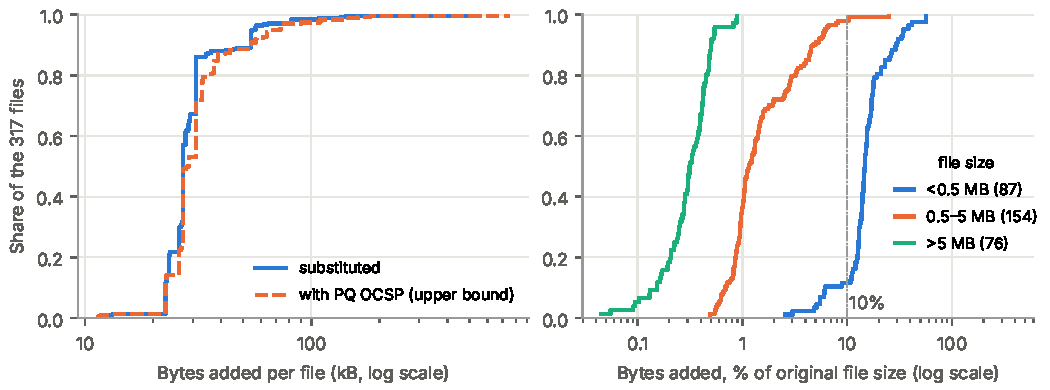
\includegraphics[width=\linewidth]{figures/corpusgrowth}
\caption{Distribution of what ML-DSA-65 would add to the \NcpqFiles{} production
files. Left: bytes added per file, as substituted and with the upper bound for
post-quantum OCSP of Table~\ref{tab:corpusstrata}. Right: bytes added as a
percentage of the original file size, by file-size band (number of files in
brackets). Both axes of growth are logarithmic.}
\label{fig:corpusgrowth}
\end{figure}

\clearpage
\section{The reporting audit}
\label{sec:supp-audit}

\subsection{Protocol}
\label{sec:auditprotocol}

\emph{Sources.} Keyword searches of the arXiv API by application area (TLS,
QUIC, IoT, embedded, 5G, DNSSEC, VPN and IKEv2, SSH, blockchain, V2X and CAN,
PKI, cloud), each combined with post-quantum terms (post-quantum, ML-KEM,
Kyber, ML-DSA, Dilithium, Falcon, SPHINCS+); Europe PMC full-text searches for
open-access journal papers (Sensors, Entropy, Scientific Reports); and web
searches for venue papers with open PDFs (NDSS MADWeb, MDPI Cryptography).
The audit was completed on 2~November 2026. The exact query strings were not logged, which a replication would have
to reconstruct from the terms above.

\emph{Inclusion.} Published 2022--2026; the study reports its own timing of a
post-quantum KEM or signature, as a primitive, a handshake or end to end, in an
applied setting; the full text could be read. Preprints count as studies:
\NauditPreprints{} of the \NauditN{} are arXiv preprints, included if first
posted before 3~September 2026, sixty days before the audit, so that a recent
preprint had time to be revised; one later preprint was kept because it had
already been accepted at a workshop (Gillot et al., QSIoT 2026). Where a paper has a published version that
could not be read, the arXiv text was coded and the version is recorded.

\emph{Exclusion and screening.} Fifty-six candidates were screened and
sixteen excluded: four whose contribution is an optimised or hardware
implementation or that report no separable timing (arXiv 2404.13544,
2606.15744, 2607.12504, 2509.11695), four whose post-quantum cost is
simulated or projected (2308.10696, 2309.03338, 2608.05087, 2604.04191), two
generic desktop benchmarks (2508.00832, 2503.12952), one without a stated
measurement method (2502.02851), one not in English (2501.07028), and four
under the recency rule (2609.23902, 2609.27828, 2610.38632, 2610.32356).

\emph{Coding.} A mark requires an explicit statement in the text; the
released file quotes the sentence or table that supports each mark and names
the version of the text coded. One author coded every study and there was no
second rater, so no agreement statistic exists; the borderline calls are
explained in the released notes.

\subsection{Studies}

{\footnotesize
\begin{longtable}{p{3.1cm}p{2.0cm}cccccccc}
\caption{Forty applied post-quantum timing studies, 2022--2026, coded for what they report about the implementation behind their numbers: library (\emph{Lib.}), its version (\emph{Ver.}), the compiler (\emph{Cc}), the build (\emph{Fl.}: \checkmark{} an explicit optimisation level such as \texttt{-O3}; ($\checkmark$) a build type or an optimised-versus-portable backend without one), CPU model and clock (\emph{CPU}), repetitions (\emph{Rep.}), a measure of spread (\emph{Spr.}) and released code or data (\emph{Code}). A mark means the paper states it explicitly. Coding by one author, without a second rater; the evidence for every mark, with the version of the text coded, is quoted in the released data (Section~\ref{sec:auditprotocol}).}\label{tab:audit}\\
\toprule
Study & Area & Lib. & Ver. & Cc & Fl. & CPU & Rep. & Spr. & Code\\
\midrule
\endfirsthead
\toprule
Study & Area & Lib. & Ver. & Cc & Fl. & CPU & Rep. & Spr. & Code\\
\midrule
\endhead
\bottomrule
\endfoot
\citet{septienhernandez2022comparative} & IoT (MQTT over Wi-Fi/\allowbreak{}LoRa gateway) & \checkmark & \checkmark &  &  &  & \checkmark & \checkmark & \\
\citet{cultice2023novel} & CAN bus (3D printer /\allowbreak{} embedded controllers) &  &  &  &  &  &  &  & \\
\citet{goertzen2023post} & DNSSEC & \checkmark & \checkmark &  &  & \checkmark &  & \checkmark & \checkmark\\
\citet{gurung2023performance} & blockchain-based federated learning & \checkmark &  &  &  &  &  &  & \\
\citet{astrizi2024seamless} & TLS 1.3 /\allowbreak{} KEMTLS with identity-based encryption & \checkmark &  &  &  &  & \checkmark & \checkmark & \checkmark\\
\citet{canoaguilera2024inline} & data-centre links (IPsec on DPUs) & \checkmark &  &  & ($\checkmark$) & \checkmark & \checkmark &  & \\
\citet{dong2024evaluating} & embedded TLS & \checkmark &  &  &  &  &  &  & \\
\citet{fitzgibbon2024constrained} & IoT (Raspberry Pi TLS and primitive benchmarks) & \checkmark & \checkmark &  &  & \checkmark & \checkmark &  & \\
\citet{kampanakis2024impact} & TLS/\allowbreak{}web (time-to-last-byte) & \checkmark &  &  &  & \checkmark & \checkmark & \checkmark & \checkmark\\
\citet{kempf2024quantum} & QUIC/\allowbreak{}TLS & \checkmark &  &  &  &  & \checkmark & \checkmark & \checkmark\\
\citet{mamun2024enhancing} & transportation CPS (Kyber over Ethernet/\allowbreak{}LTE) & \checkmark &  &  &  &  & \checkmark & \checkmark & \\
\citet{shah2024double} & DNSSEC (double signatures) & \checkmark & \checkmark &  &  &  & \checkmark &  & \\
\citet{buruaga2025hybrid} & TLS over SDN/\allowbreak{}QKD &  &  &  &  &  & \checkmark &  & \\
\citet{chen2025security} & TLS 1.3 hybrid key exchange & \checkmark & \checkmark &  &  &  & \checkmark & \checkmark & \checkmark\\
\citet{conti2025pq} & automotive (CAN bus, emulated ECUs) &  &  &  & ($\checkmark$) &  & \checkmark &  & \checkmark\\
\citet{dai2025lightweight} & V2X key agreement (Veins/\allowbreak{}OMNeT++) & \checkmark &  &  & ($\checkmark$) &  & \checkmark & \checkmark & \\
\citet{gentosuela2025implementing} & DNSSEC (CoreDNS) & \checkmark & \checkmark & \checkmark &  & \checkmark & \checkmark & \checkmark & \checkmark\\
\citet{hoque2025analysis} & 5G UE-to-UE TLS & \checkmark &  &  &  &  & \checkmark &  & \checkmark\\
\citet{lee2025quantum} & DNS (DoT/\allowbreak{}DoH, DNSSEC) & \checkmark & \checkmark &  &  & \checkmark & \checkmark &  & \checkmark\\
\citet{lopez2025evaluating} & IoT (Raspberry Pi KEM exchange) & \checkmark & \checkmark &  &  &  &  & \checkmark & \checkmark\\
\citet{patterson2025energy} & embedded (key generation energy) & \checkmark & \checkmark &  &  &  & \checkmark &  & \checkmark\\
\citet{schemitt2025assessing} & blockchain (Bitcoin/\allowbreak{}Ethereum simulation) & \checkmark & \checkmark &  &  &  & \checkmark & \checkmark & \checkmark\\
\citet{tadepalli2025impact} & TLS/\allowbreak{}web & \checkmark &  &  &  &  &  & \checkmark & \\
\citet{tsili2025scalable} & PKI (CA hierarchy, certificate issuance) & \checkmark &  &  &  & \checkmark &  &  & \\
\citet{balaji2026operationalising} & financial infrastructure TLS (web server + Java API gateway) & \checkmark &  &  &  &  &  & \checkmark & \\
\citet{chopra2026pqc} & 5G core (cloud-native, Kubernetes) & \checkmark &  & \checkmark &  &  & \checkmark & \checkmark & \\
\citet{chou2026network} & TLS/\allowbreak{}PKI (certificate chains) & \checkmark &  &  &  &  & \checkmark & \checkmark & \checkmark\\
\citet{commey2026performance} & consumer electronics /\allowbreak{} IoT & \checkmark & \checkmark & \checkmark & \checkmark & \checkmark & \checkmark & \checkmark & \checkmark\\
\citet{commey2026pqs} & blockchain-based federated learning & \checkmark &  &  &  &  &  &  & \checkmark\\
\citet{feingold2026mqtt} & IoT (MQTT) & \checkmark &  &  &  &  & \checkmark &  & \checkmark\\
\citet{gillot2026energy} & embedded and general-purpose (energy) & \checkmark & \checkmark &  &  & \checkmark & \checkmark &  & \checkmark\\
\citet{gillot2026testing} & IoT/\allowbreak{}embedded TLS & \checkmark &  &  &  & \checkmark & \checkmark & \checkmark & \checkmark\\
\citet{gomezcambronero2026layered} & TLS & \checkmark & \checkmark &  &  &  & \checkmark & \checkmark & \checkmark\\
\citet{hoque2026energy} & 5G user equipment TLS & \checkmark &  &  &  &  & \checkmark &  & \\
\citet{jain2026performance} & blockchain prototype & \checkmark &  & \checkmark & ($\checkmark$) &  & \checkmark &  & \checkmark\\
\citet{kudaloor2026quantum} & 6G /\allowbreak{} TLS & \checkmark & \checkmark &  &  &  & \checkmark &  & \\
\citet{latah2026ovs} & SDN (OVS southbound TLS) & \checkmark & \checkmark &  &  &  & \checkmark &  & \\
\citet{liu2026drop} & SSH (KEM-based client authentication) & \checkmark & \checkmark & \checkmark & \checkmark & \checkmark & \checkmark & \checkmark & \checkmark\\
\citet{perera2026quantum} & 5G O-RAN IPsec (E2 interface) & \checkmark & \checkmark &  &  & \checkmark & \checkmark & \checkmark & \\
\citet{rassekhnia2026quantum} & IoT (MQTT/\allowbreak{}HTTP/\allowbreak{}HTTPS on ESP32) &  &  &  &  &  &  &  & \\
\end{longtable}

}

\clearpage
\bibliographystyle{ACM-Reference-Format}
\bibliography{refs,audit}

\end{document}
